\documentclass[a4paper]{article}
\usepackage{graphicx}
\usepackage[left=3.18cm, right=3.18cm, top=2.54cm, bottom=2.54cm]{geometry}
\usepackage{fancyhdr}
\usepackage{setspace}
\usepackage{amsmath}
\usepackage{amssymb}
\usepackage{booktabs}
\usepackage{colortbl}
\usepackage{xcolor}
\usepackage{subcaption}
\usepackage{grffile}

\newcommand{\minval}[1]{\textbf{\textcolor{red}{#1}}}

\pagestyle{fancy}
\lhead{} % Clear left header
\chead{ESE5004 - Midterm Report} % Center header
\rhead{} % Clear right header
\onehalfspacing
\setlength{\parindent}{0pt}
\setlength{\parskip}{1em}

\begin{document}
\begin{titlepage}
    \centering
    \vspace*{-2.5cm}
    \includegraphics[width=0.75\textwidth]{../attachment/nus.jpg} \\
    \Huge
    \textbf{Midterm Report}

    \vspace{1.5cm}
    \Large
    \textbf{Topic:} Application of Supervised Learning Methods to Transformation Mechanisms in DBPs Formation in simulated drinking water distribution network

    \vspace{1.5cm}
    \textbf{Name:} Zhou Dafu \\
    \textbf{Number:} A0331761J

    \vspace{1cm}
    \textbf{Supervisor:} Prof. Hu Jiangyong \\
    \textbf{Mentor:} Mr. Sun Yuanpeng

    \vfill
    \Large
    \date{\today}
\end{titlepage}

\section{Introduction}

\subsection{Background}
Disinfection is a critical step in municipal water treatment, designed to eliminate pathogenic microorganisms and ensure public health. However, chemical disinfectants, most commonly chlorine, react with naturally occurring organic matter (NOM) and other precursors in the water to form a wide array of unintended compounds known as disinfection by-products (DBPs)~\cite{galliard2004organic}. Many DBPs are of health concern due to their potential carcinogenic and mutagenic properties~\cite{siddique2012review}. Consequently, water utilities face the challenge of balancing microbial safety with the minimization of DBP formation.

Predicting DBP concentrations within complex water distribution systems (WDS) is a significant challenge due to dynamic hydraulic conditions and complex chemical kinetics. Traditional monitoring relies on infrequent grab sampling and laboratory analysis, which is costly and provides low temporal resolution. This research aims to leverage high-frequency sensor data and supervised machine learning techniques to develop predictive models for DBP indicators, such as Total Residual Chlorine (TRC), Total Organic Carbon (TOC), and pH. The successful development of these models would enable proactive operational control to mitigate DBP formation and improve water quality management. This report outlines the progress made in data preprocessing, model selection, and experimental design for this purpose.

\subsection{DBP Formation Chemistry}
The formation of Disinfection By-Products (DBPs) in this system is a multi-step process governed by the interactions between disinfectants and precursors under alkaline conditions. The process begins with the formation of monochloramine ($NH_2Cl$), which serves as the primary disinfectant. In the presence of ammonium ions ($NH_4^+$) and hypochlorite ions ($OCl^-$), which are the dominant species in the alkaline environment created by slaked lime, monochloramine is produced according to the following total reaction:
\begin{equation}
    \text{NH}_3 + \text{OCl}^- \rightarrow \text{NH}_2\text{Cl} + \text{OH}^-
\end{equation}
Once formed, chloramines can react with organic nitrogen precursors (e.g., secondary amines) present in the water. This reaction typically involves the formation of intermediate compounds, such as chlorinated unsymmetrical dialkylhydrazines. These intermediates are subsequently oxidized by dissolved oxygen to form nitrogenous DBPs (N-DBPs), such as nitrosamines (e.g., N-nitrosodimethylamine, NDMA)~\cite{hua2015formation}. This pathway highlights the critical role of chloramine speciation and the presence of organic precursors in the generation of potentially harmful by-products.

\subsection{Deep Learning in Water Engineering}
Deep learning has emerged as a powerful tool in water engineering, offering new capabilities for modeling complex, non-linear systems that are difficult to capture with traditional mechanistic models. In the context of water quality, deep learning models can leverage high-frequency sensor data to predict critical parameters, detect anomalies, and optimize treatment processes. This study aims to bridge the gap between traditional water chemistry and modern data-driven approaches by applying advanced neural network architectures to the problem of DBP prediction.

\subsection{Model Architectures}
To capture the complex, non-linear dynamics of DBP formation, several neural network architectures are considered for this regression task, as illustrated in Figures \ref{fig:mlp_structure} through \ref{fig:gru_structure}:
\begin{itemize}
    \item \textbf{Multilayer Perceptron (MLP):} A foundational feedforward neural network that can model complex non-linear relationships. It consists of an input layer, one or more hidden layers, and an output layer. Each layer contains neurons that are fully connected to the neurons in the subsequent layer. In addition to accepting single data points as input, the MLP architecture in this study was also adapted to process time-series data. This variant, referred to as MLPHIS, flattens a fixed-length window of historical time-series data into a single vector, which is then fed into the network. This allows the MLP to capture some temporal patterns without recurrent connections.
    \item \textbf{Recurrent Neural Network (RNN):} Designed to handle sequential data by maintaining a hidden state that captures past information. The output at a given time step is a function of the current input and the hidden state from the previous time step. This recurrent connection allows RNNs to model temporal dependencies, but they can struggle with long-term dependencies due to the vanishing gradient problem.
    \item \textbf{Long Short-Term Memory (LSTM):} A specialized RNN architecture that uses gating mechanisms (input, forget, and output gates) to overcome the vanishing gradient problem and effectively learn long-term dependencies~\cite{hochreiter1997long}. The gates control the flow of information, allowing the network to selectively remember or forget information over long sequences, making it well-suited for time-series forecasting.
    \item \textbf{Gated Recurrent Unit (GRU):} A simplified version of the LSTM with fewer parameters, which often performs comparably on many tasks. It combines the input and forget gates into a single "update gate" and merges the cell state and hidden state. This makes the GRU more computationally efficient than the LSTM while still retaining its ability to capture long-term dependencies.
\end{itemize}

\begin{figure}[h!]
    \centering
    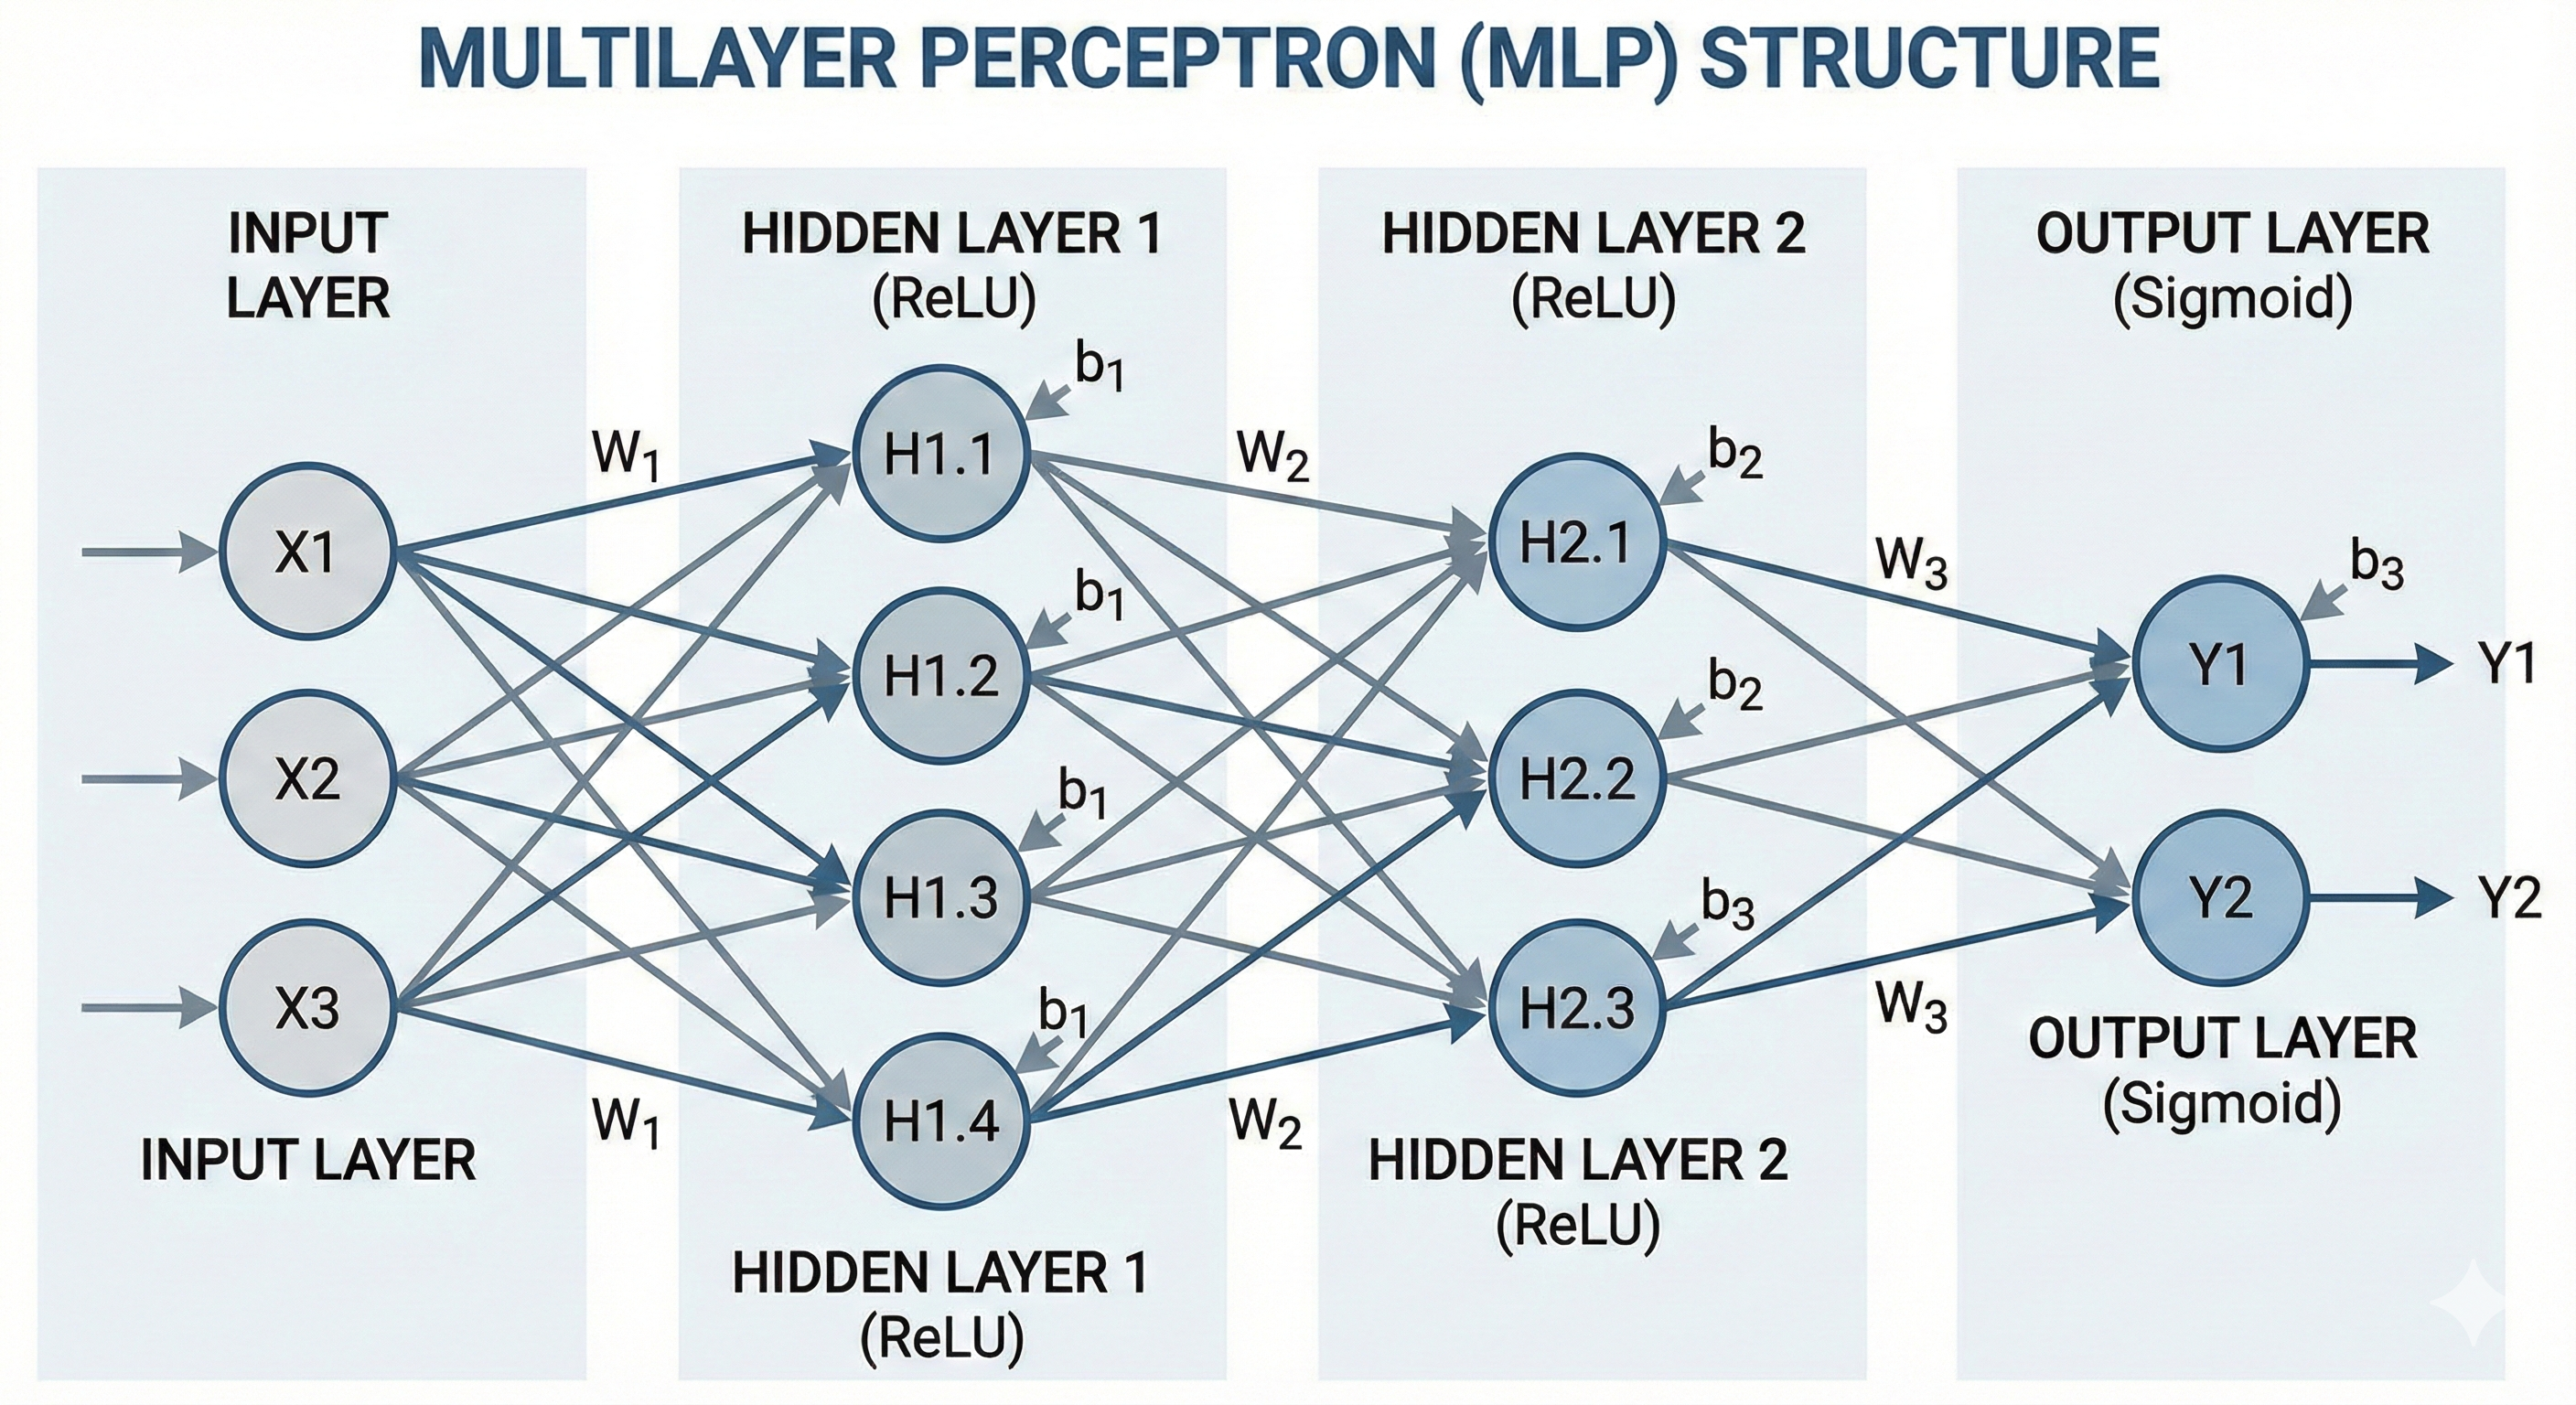
\includegraphics[width=0.6\textwidth]{../attachment/mlp.png}
    \caption{Structure of a Multilayer Perceptron.}
    \label{fig:mlp_structure}
\end{figure}

\begin{figure}[h!]
    \centering
    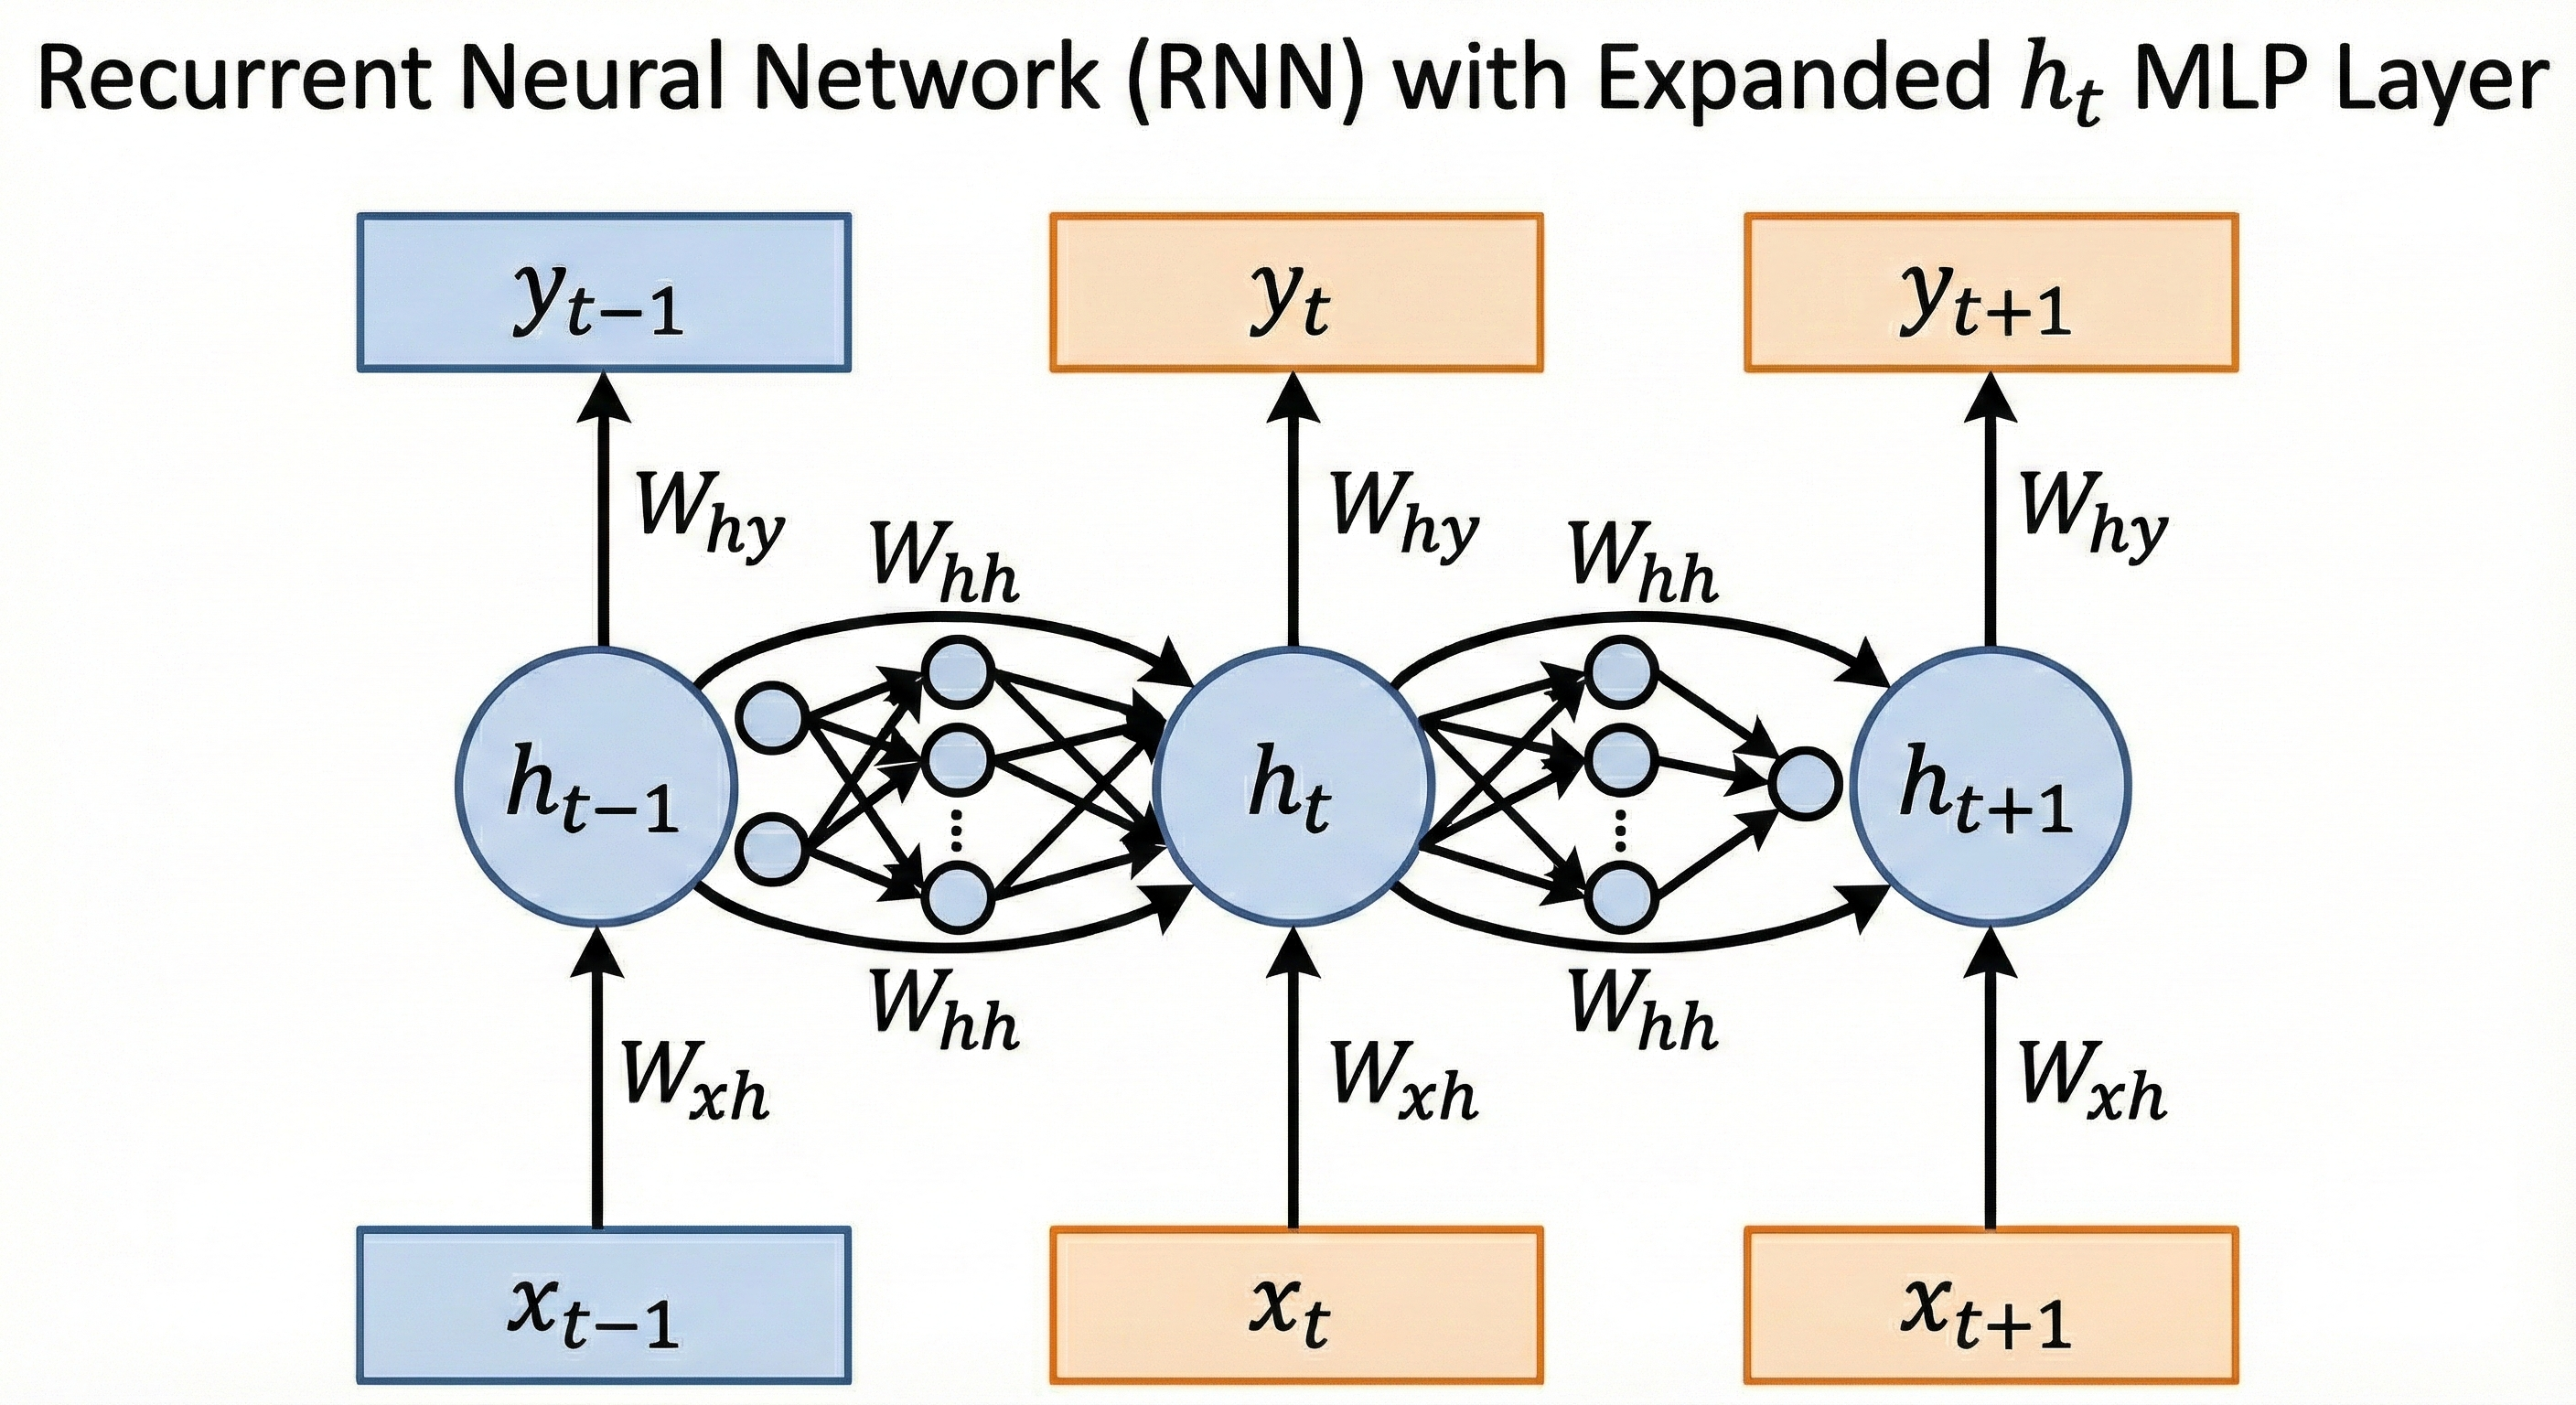
\includegraphics[width=0.7\textwidth]{../attachment/rnn.png}
    \caption{Structure of a Recurrent Neural Network.}
    \label{fig:rnn_structure}
\end{figure}

\begin{figure}[h!]
    \centering
    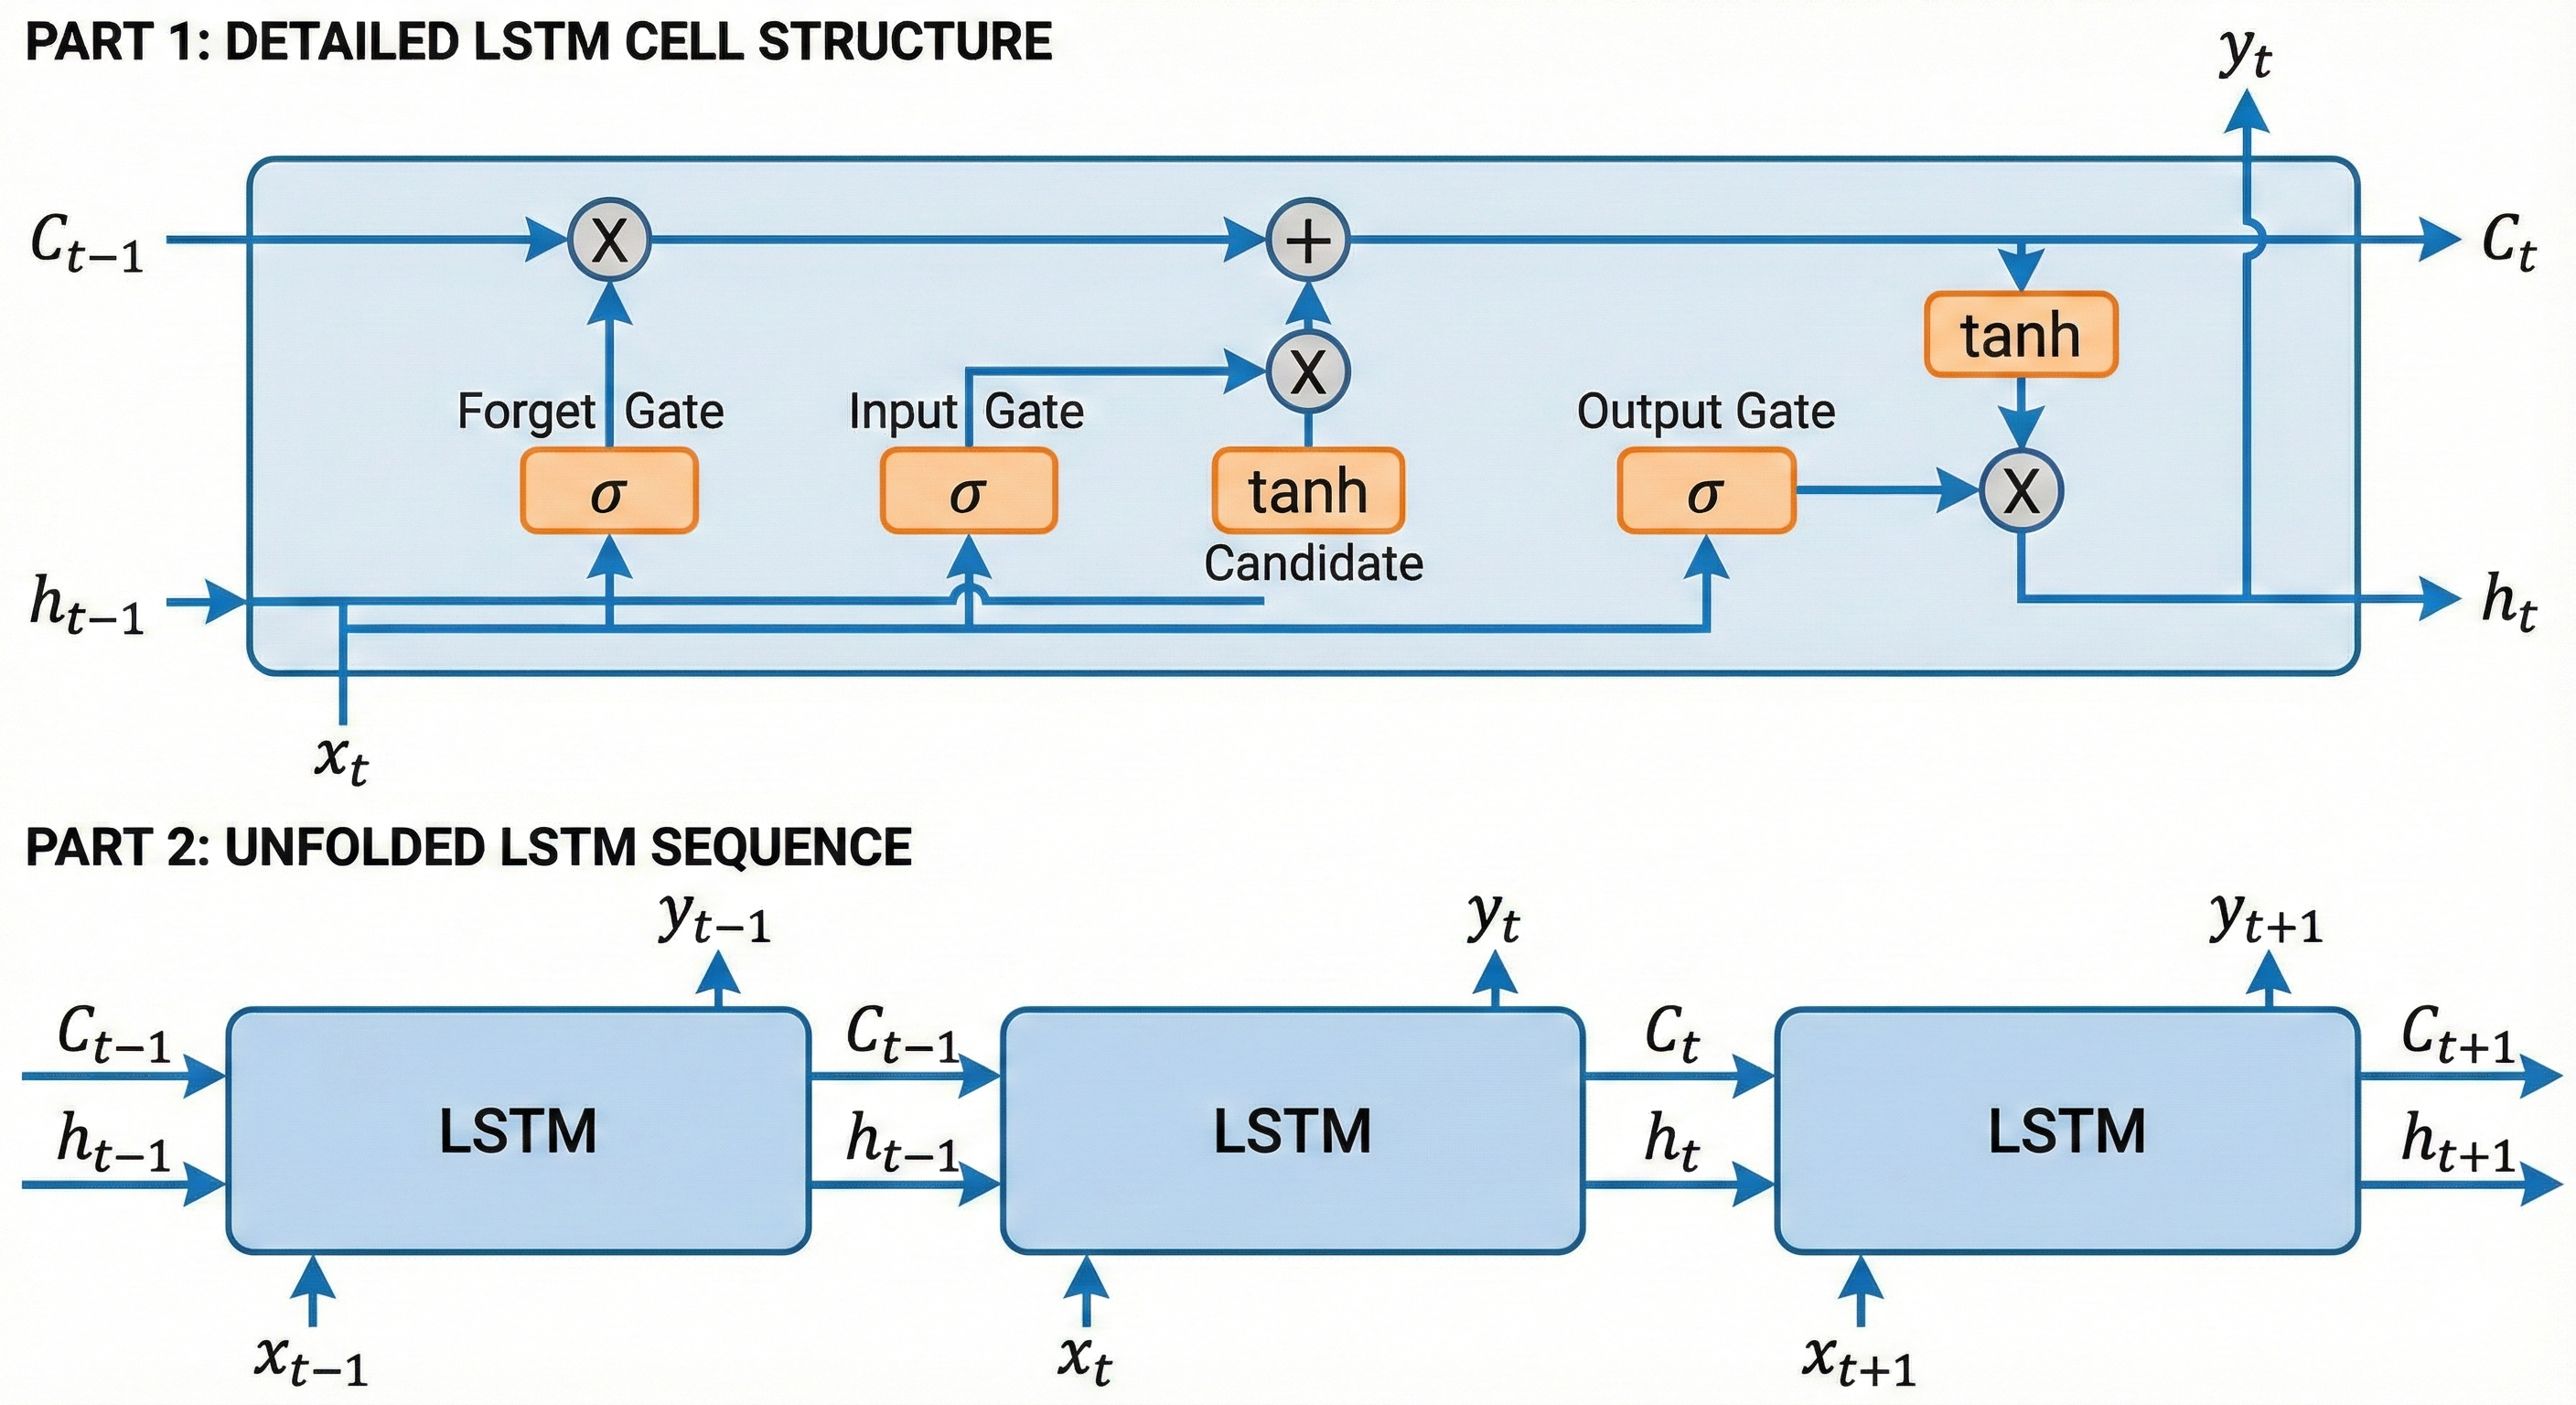
\includegraphics[width=0.7\textwidth]{../attachment/lstm.png}
    \caption{Structure of a Long Short-Term Memory Cell.}
    \label{fig:lstm_structure}
\end{figure}

\begin{figure}[h!]
    \centering
    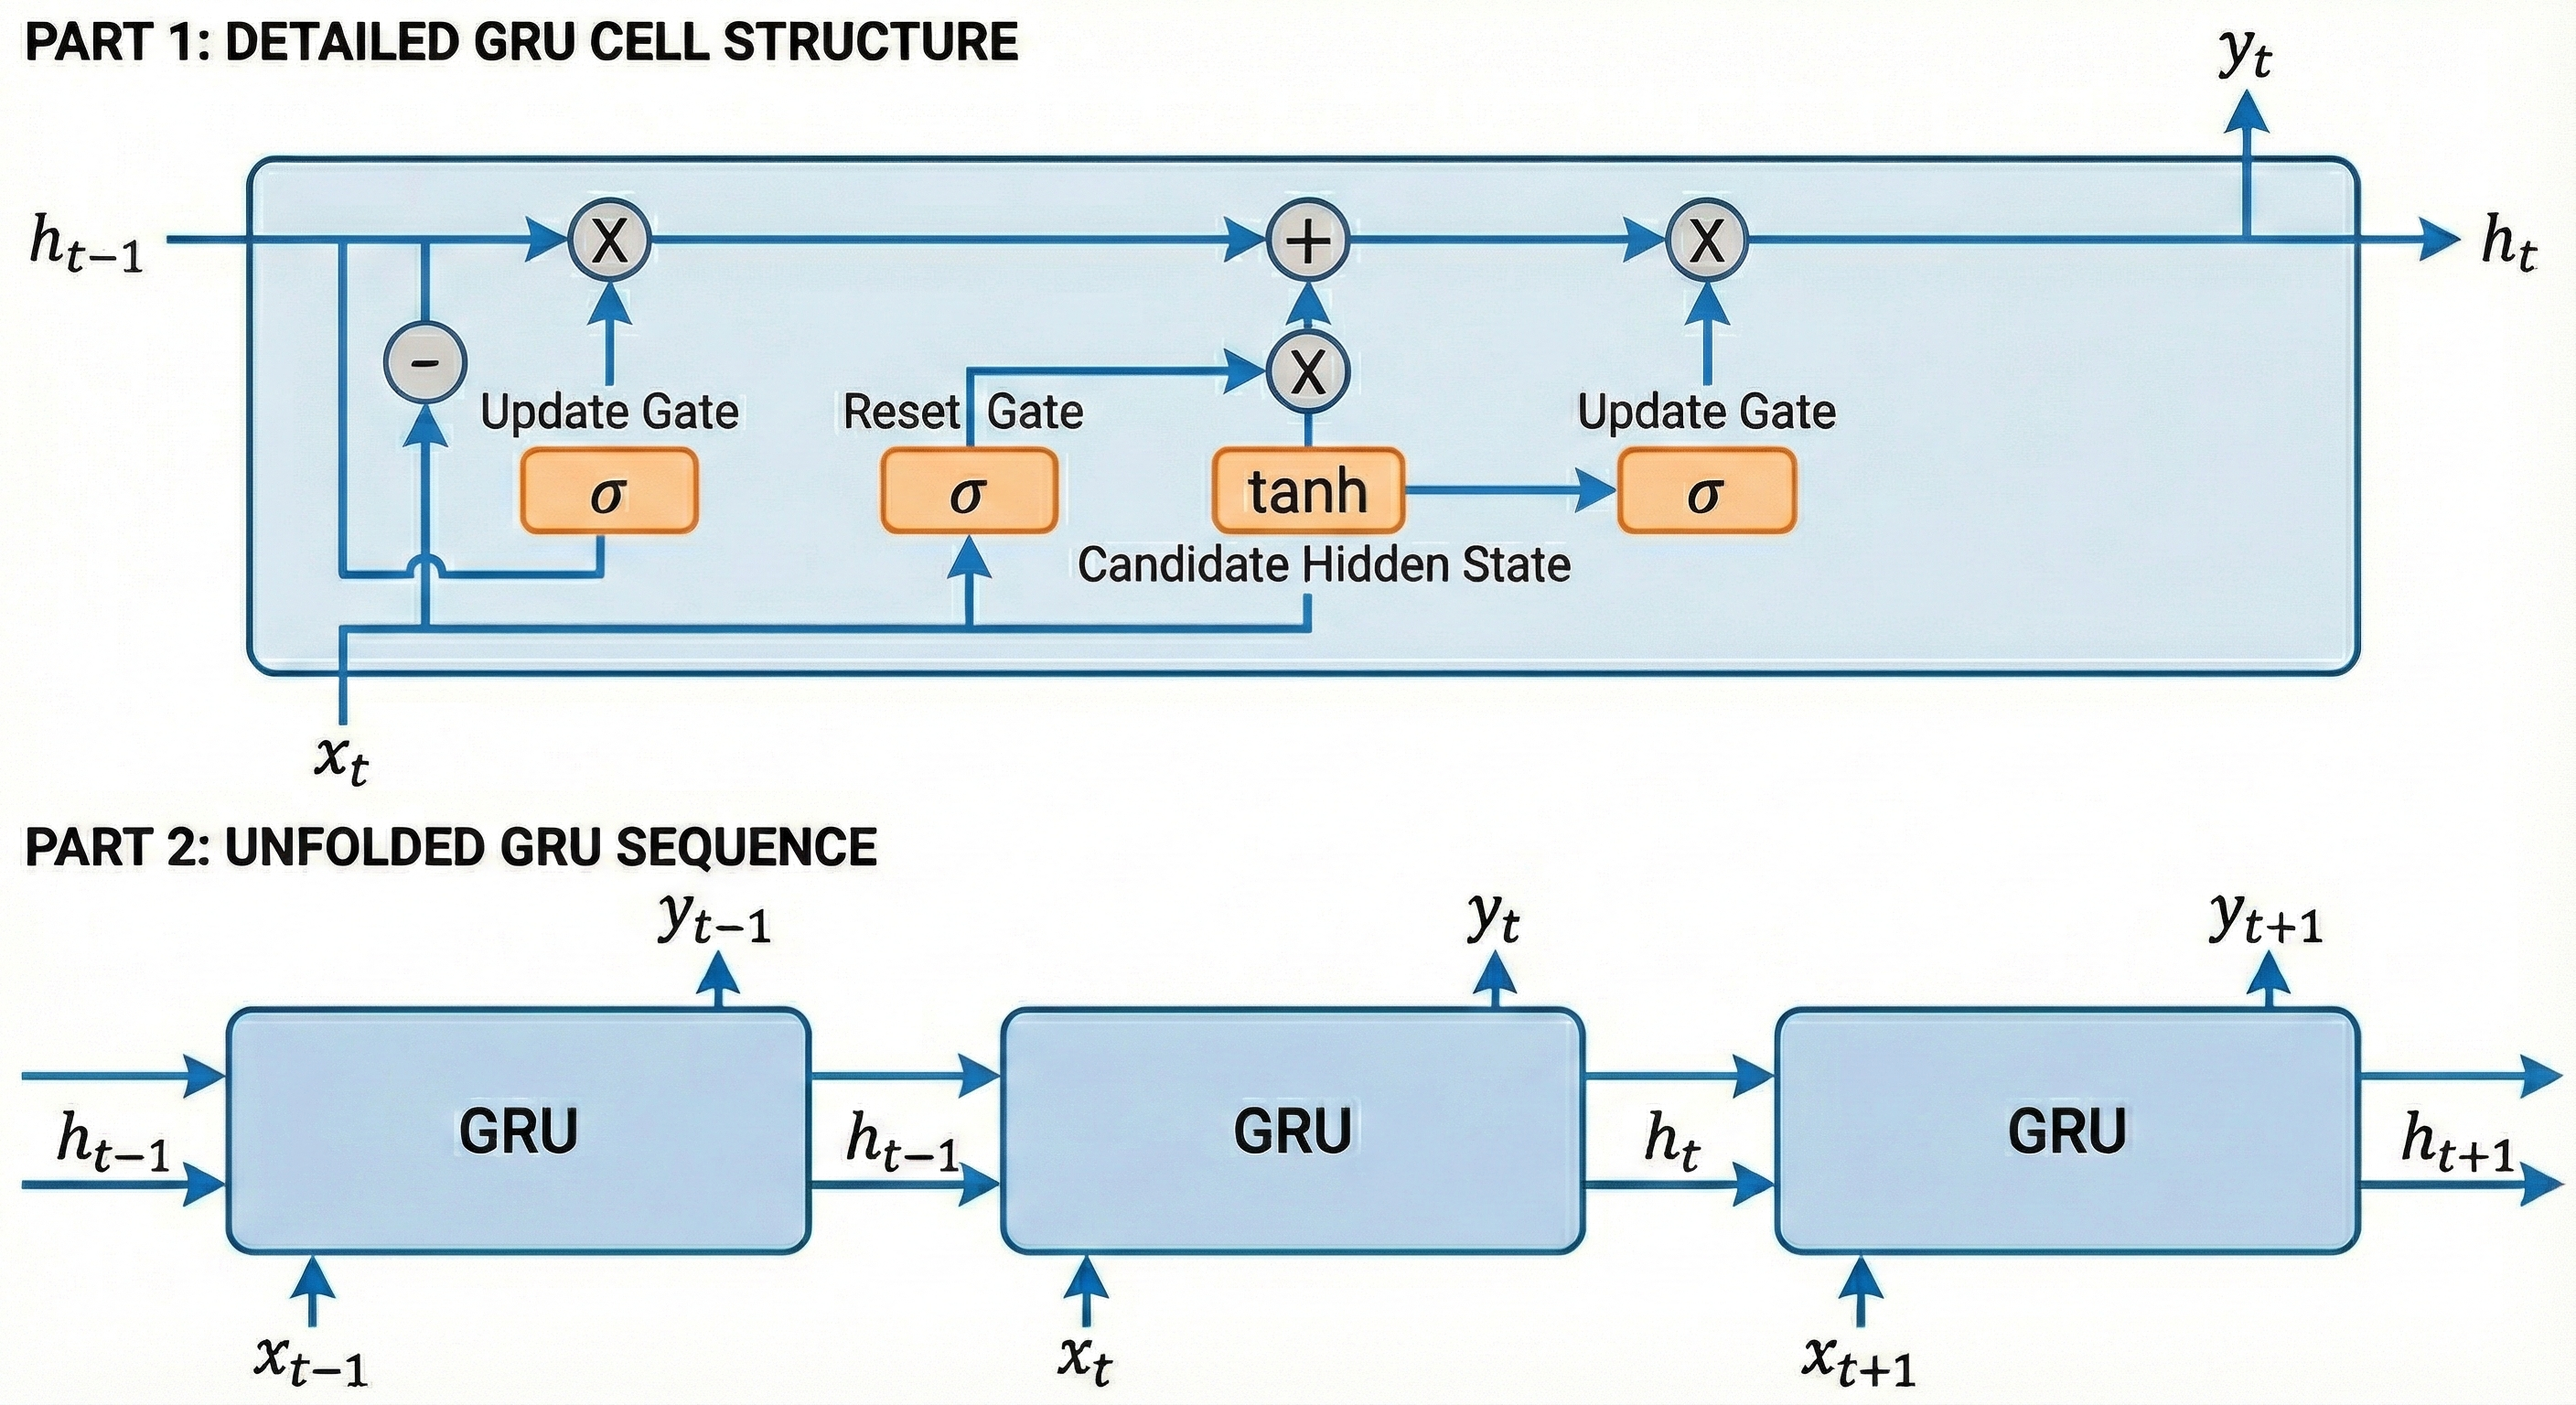
\includegraphics[width=0.7\textwidth]{../attachment/gru.png}
    \caption{Structure of a Gated Recurrent Unit Cell.}
    \label{fig:gru_structure}
\end{figure}
\section{Objectives}
The primary objectives of this study are:
\begin{enumerate}
    \item To evaluate the performance of various deep learning architectures (MLP, RNN, LSTM, GRU) in predicting water quality parameters from sensor data.
    \item To investigate the correlation between high-frequency sensor measurements (TRC, pH, TOC, etc.) and DBP formation.
    \item To establish a robust machine learning framework for predicting DBP concentrations based on readily available sensor data, thereby enabling real-time monitoring and control.
\end{enumerate}

\section{Methodology}

\subsection{System Description and Data Acquisition}
The study focuses on a section of a water distribution system comprising five main stages, as illustrated in Figure \ref{fig:reactors}:
\begin{enumerate}
    \item \textbf{Feed Water Tank (FWT):} Raw water storage before post-treatment. Not included in the modeling.
    \item \textbf{Disinfection Tank (DT):} Where disinfection chemicals are introduced and mixed.
    \item \textbf{Retention Tank (RT):} Storage before water supply.
    \item \textbf{Pipeline 1 (PPL1):} Upper stream of distribution network.
    \item \textbf{Pipeline 2 (PPL2):} Lower stream of distribution network.
\end{enumerate}

\begin{figure}[h!]
\centering
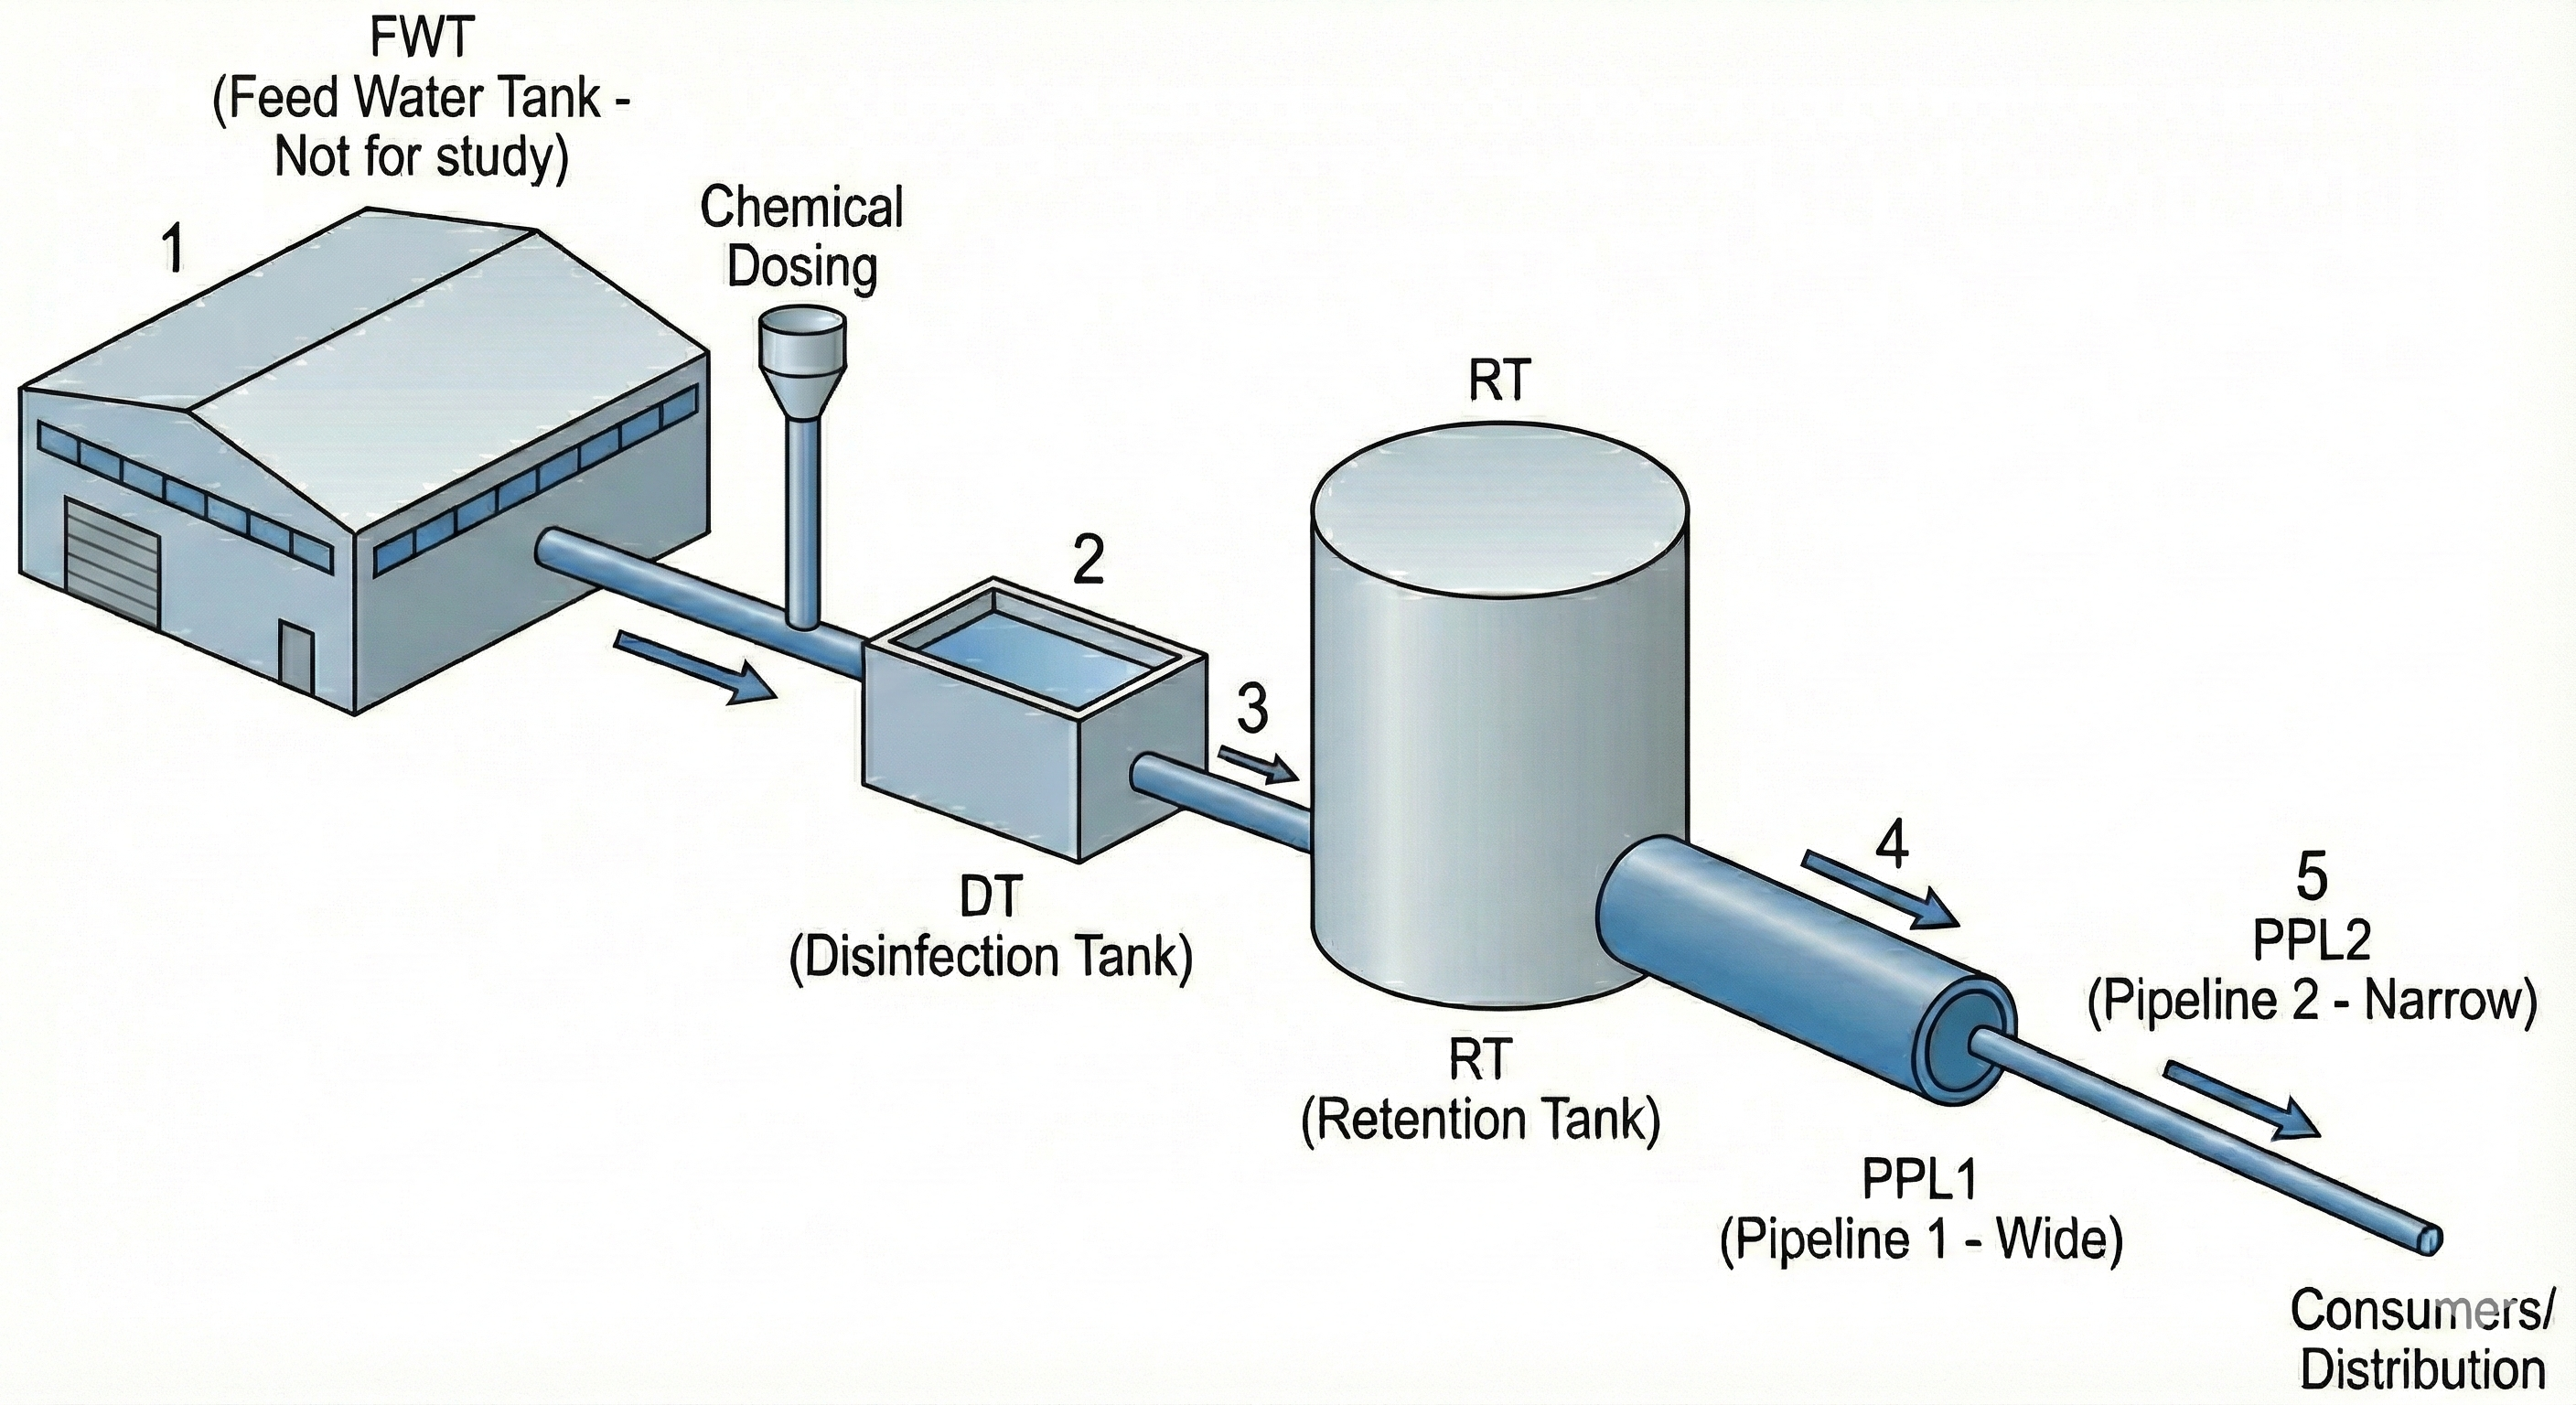
\includegraphics[width=0.8\textwidth]{../attachment/reactors.png}
\caption{Schematic of the reactor flow process in the water distribution system.}
\label{fig:reactors}
\end{figure}

Water quality data is collected via multi-parameter sensors at different stages. The parameters include Total Residual Chlorine (TRC), pH, Conductivity, Fluorescent Dissolved Organic Matter (fDOM), Dissolved Oxygen (DO), Total Organic Carbon (TOC), and Dissolved Organic Carbon (DOC). Data is recorded at a 5-minute interval. The availability of sensor measurements at each stage is summarized in Table \ref{tab:sensor_data}.

\begin{table}[h!]
\centering
\caption{Availability of Sensor Measurements at Each Stage}
\label{tab:sensor_data}
\begin{tabular}{lcccc}
\toprule
\textbf{Parameter} & \textbf{DT} & \textbf{RT} & \textbf{PPL1} & \textbf{PPL2} \\
\midrule
TRC & \checkmark & \checkmark & \checkmark & \checkmark \\
pH & \checkmark & \checkmark & \checkmark & \checkmark \\
Conductivity & \checkmark & \checkmark & \checkmark & \checkmark \\
fDOM (QSU) &  & \checkmark & \checkmark & \checkmark \\
DO &  & \checkmark & \checkmark & \checkmark \\
TOC &  & \checkmark & \checkmark & \checkmark \\
DOC &  & \checkmark & \checkmark & \checkmark \\
\bottomrule
\end{tabular}
\end{table}

\subsection{Data Preprocessing}

\subsubsection{Imputation of Missing Values}
A unique challenge in the dataset arises from the measurement setup for PPL1 and PPL2, where a single sensor alternates between the two locations every 30 minutes. This results in blocks of six consecutive missing values for each pipeline stage, alternating with six valid measurements. To create a continuous time series for model training, these missing values must be imputed.

The imputation process is as follows, with a visual representation in Figure \ref{fig:imputation_example}. For a block of missing data with available data segments both before and after, a two-step approach is used. First, linear regression models are fitted to the data segments preceding and succeeding the gap. The initial imputed values are determined by creating a linear interpolation between the predicted value at the end of the preceding segment and the predicted value at the beginning of the succeeding segment. Subsequently, random noise is added to these initial values. The variance of this noise is set to the smaller of the variances from the two fitted linear regression models, preserving the statistical properties of the local time series. In cases where a missing data block is at the beginning or end of the dataset, only the nearest available data segment is used. A linear regression model is fitted to this segment, and the resulting regression line is extrapolated to fill the missing values. Random noise, with a variance equal to that of the regression model, is then added to these extrapolated values.

\begin{figure}[h!]
\centering
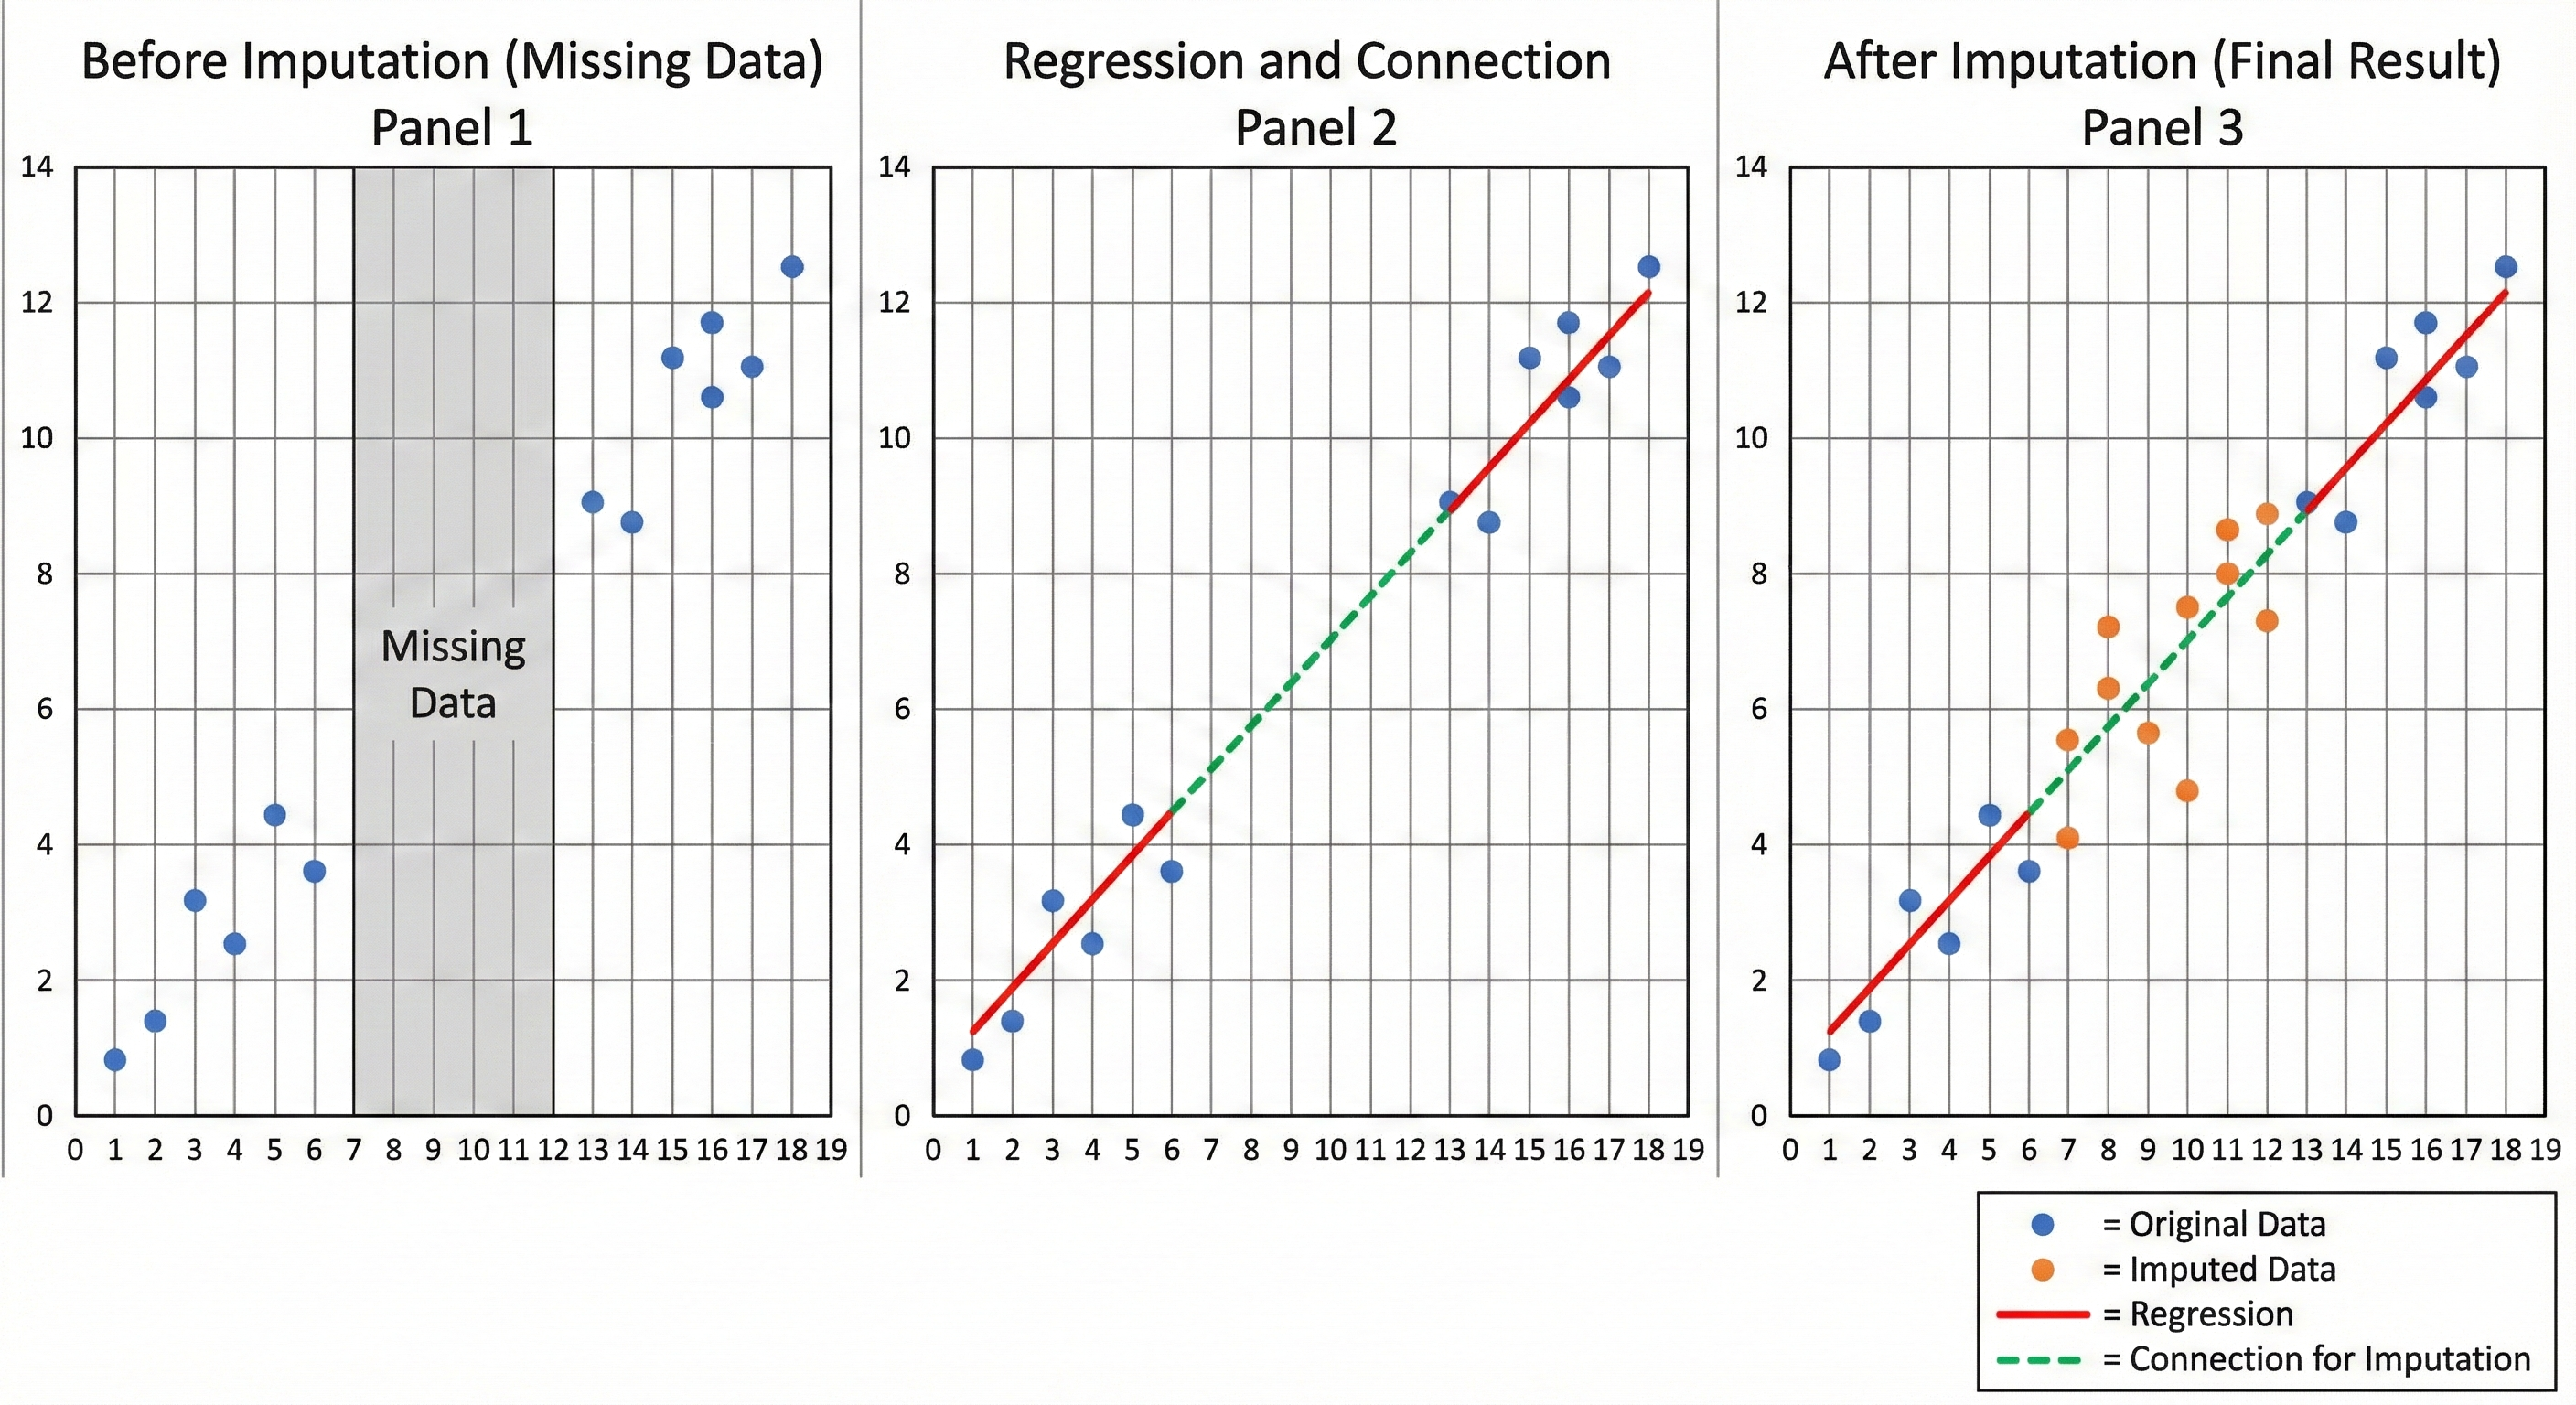
\includegraphics[width=0.8\textwidth]{../attachment/imputation.png}
\caption{Conceptual Example of Missing Value Imputation.}
\label{fig:imputation_example}
\end{figure}

\subsubsection{Time Alignment}
As a parcel of water flows through the WDS, there is a travel time (hydraulic delay) between consecutive stages. To model the chemical transformations accurately, the input data (from DT and RT) must be time-aligned with the output data (from PPL1 and PPL2) to ensure the model learns the relationship between the same parcel of water at different points in time. This process is conceptually illustrated in Figure \ref{fig:alignment_example}. It involves calculating the time lag between stages and shifting the data series accordingly before creating input-output pairs for the models.

\begin{figure}[h!]
\centering
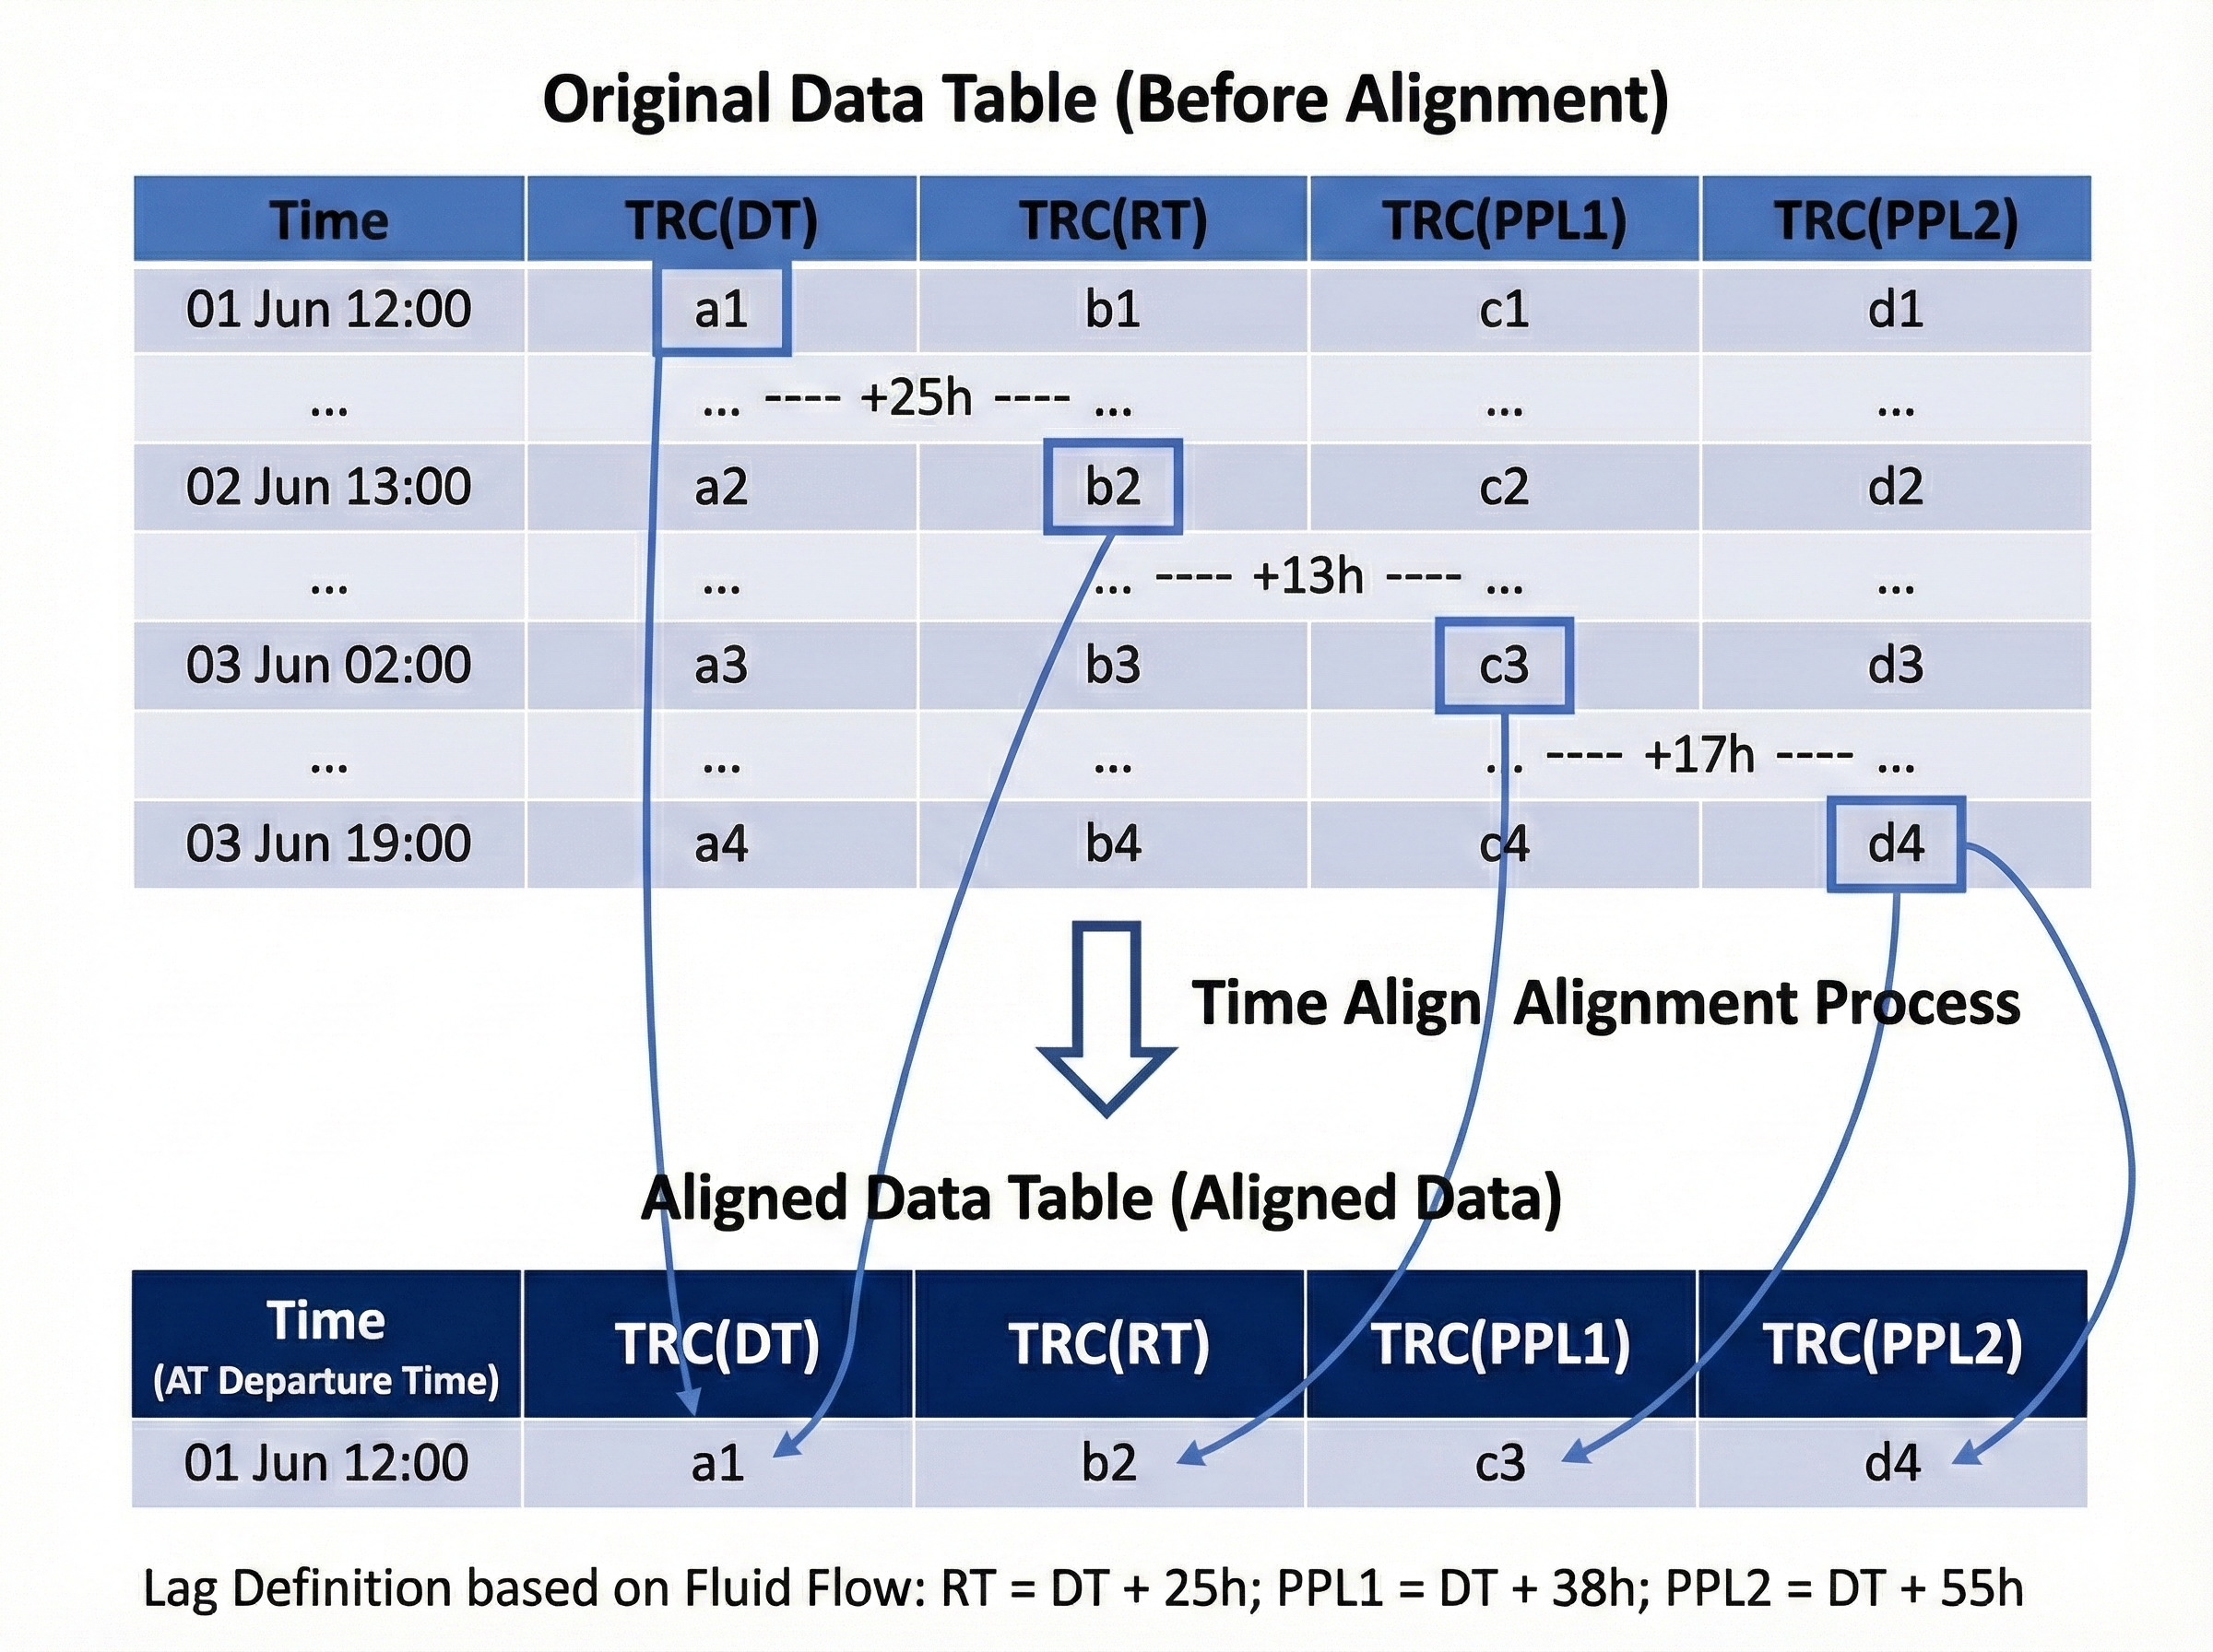
\includegraphics[width=0.8\textwidth]{../attachment/alignment.png}
\caption{Conceptual Example of Time Alignment.}
\label{fig:alignment_example}
\end{figure}

\subsection{Experiment Design and Improvements}

\subsubsection{Initial Multi-Output Approach}
The initial experimental design involved a single model with multiple output heads to simultaneously predict all target variables for PPL1 and PPL2, using sensor data from DT and RT as input. While straightforward, this approach can be suboptimal if the target variables have different scales or underlying complexities.

\subsubsection{Normalized Rate of Change Regression}
An alternative approach, termed "rate" regression, was explored to improve model sensitivity to small variations. Instead of predicting the absolute downstream concentration, the model is trained to predict a normalized rate of change. This "rate" is defined as the relative change from the upstream concentration:
\[ \text{Rate} = \frac{Y_{\text{downstream}} - Y_{\text{upstream}}}{Y_{\text{upstream}}} \]
This can be intuitively understood as the percentage by which the concentration has increased or decreased. The primary motivation for this transformation is that the absolute concentrations between upstream and downstream points often change very little. When training on absolute values, the large, relatively stable upstream value can dominate the input features, saturating the neural network's weights and making it difficult for the model to learn the small but significant variations that occur downstream. By transforming the target variable into a normalized rate, the model can focus specifically on capturing these subtle changes, leading to a more effective representation of the system's dynamics.

\subsubsection{Decoupled Model for TRC}
Preliminary experiments indicated that TRC is particularly challenging to predict accurately, yet it is a crucial driver of DBP formation. To address this, a decoupled modeling strategy was designed. One model is trained exclusively to predict TRC, allowing for a more focused architecture and hyperparameter search. A second, multi-output model is then trained to predict the remaining, less-critical parameters. This specialization is hypothesized to yield better overall predictive accuracy.

\subsection{Model Training}
The models will be trained using standard deep learning principles. The process involves feeding the model with input-output pairs and optimizing its internal weights to minimize a loss function, which quantifies the error between the model's predictions and the true values.

\begin{figure}[h!]
    \centering
    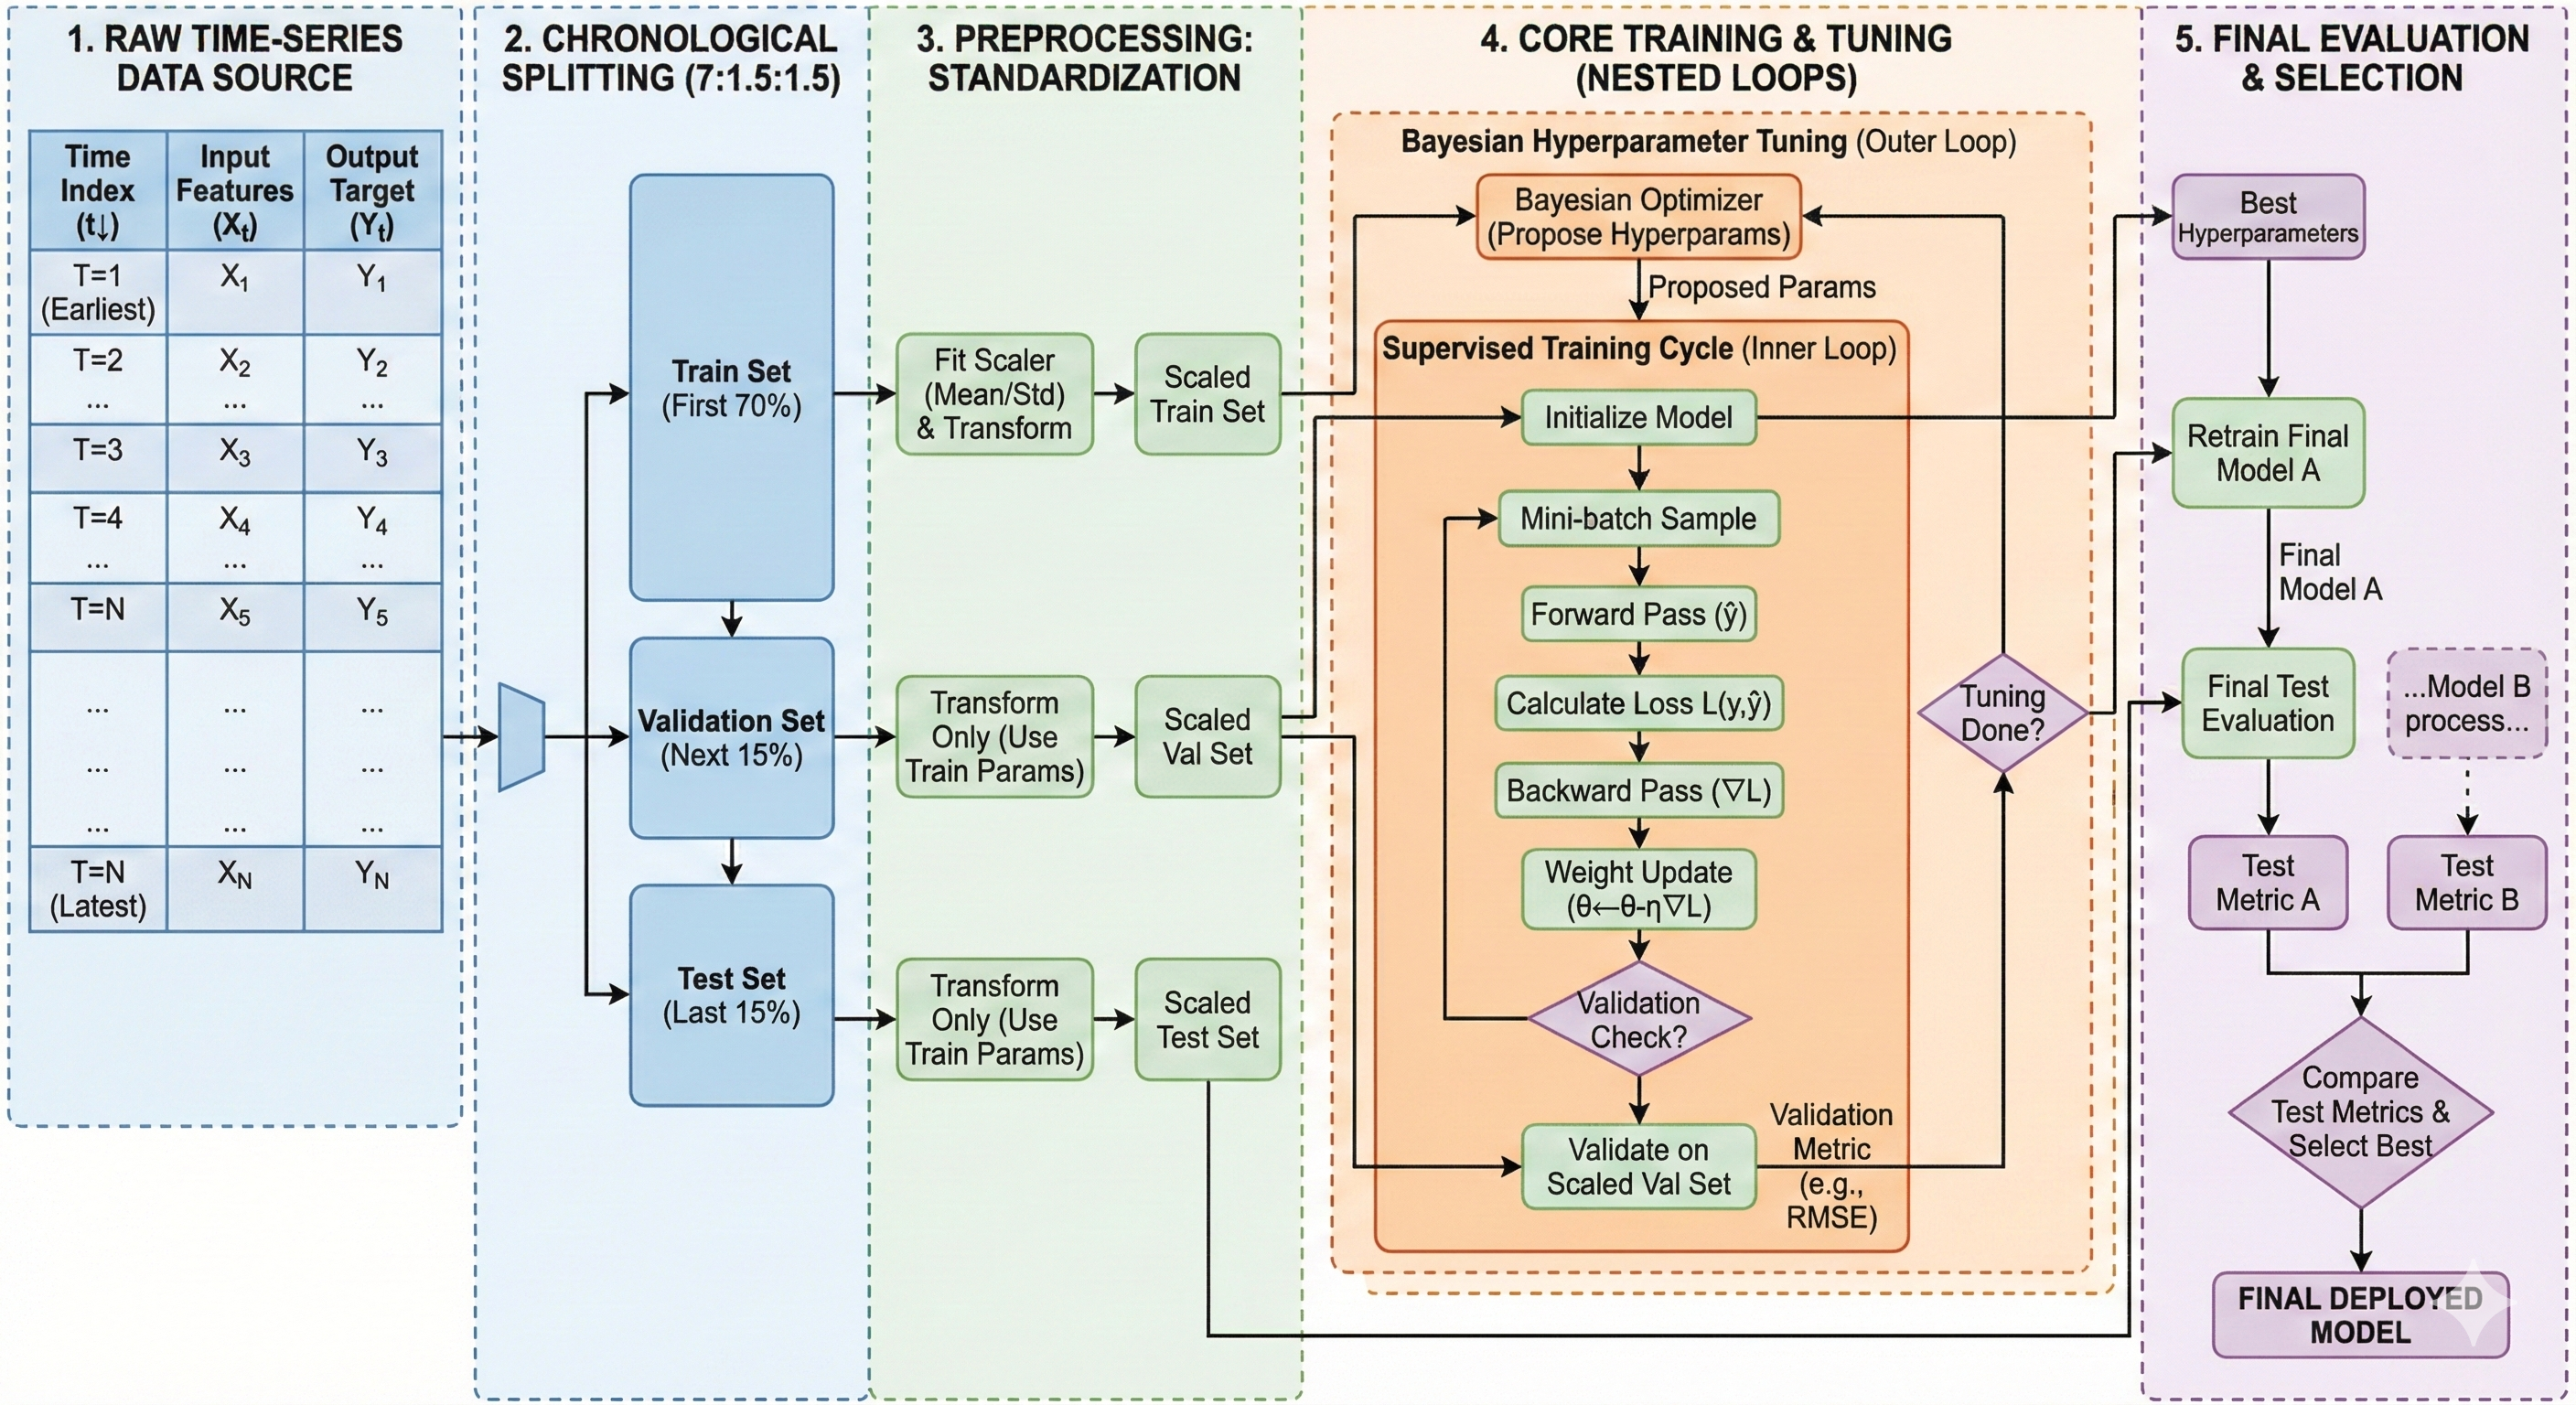
\includegraphics[width=\textwidth]{../attachment/model workflow.png}
    \caption{Model Training and Evaluation Workflow.}
    \label{fig:training_flowchart}
\end{figure}

\begin{itemize}
    \item \textbf{Loss Function:} Mean Squared Error (MSE) is chosen as the loss function, suitable for regression tasks.
    \item \textbf{Optimization:} The Adam optimizer~\cite{kingma2014adam}, an adaptive learning rate optimization algorithm, is used to update the model weights via backpropagation.
    \item \textbf{Dataset Splitting:} The data is split into training, validation, and test sets. The model learns from the training set, its hyperparameters are tuned based on performance on the validation set, and its final performance is evaluated on the unseen test set.
    \item \textbf{Regularization:} To prevent overfitting, techniques like Dropout~\cite{srivastava2014dropout} are used. Additionally, an early stopping mechanism is implemented: training is halted if the validation loss does not improve for a specified number of epochs, and the model with the best validation performance is saved.
\end{itemize}

\subsection{Hyperparameter Optimization}
The performance of neural networks is highly sensitive to the choice of hyperparameters. Key hyperparameters include learning rate, batch size, dropout rate, number of layers, number of units per layer, and the history length for sequential models. While methods like grid search and random search~\cite{bergstra2012random} exist, this project employs \textbf{Bayesian Optimization}~\cite{snoek2012practical}. Bayesian optimization builds a probabilistic model of the objective function (e.g., validation loss) and uses it to intelligently select the most promising hyperparameters to evaluate next. This approach is more efficient than exhaustive or random searches, often finding better hyperparameter configurations in fewer iterations.

\section{Results}
This section presents the quantitative results from the different modeling approaches. The performance of each model is evaluated using Mean Squared Error (MSE) and Mean Absolute Error (MAE). The results for predicting TRC, pH, and TOC at the PPL2 stage are summarized in Table \ref{tab:results_combined}.

\begin{table}[h!]
\centering
\caption{Performance Metrics for TRC, pH, and TOC Prediction at PPL2}
\label{tab:results_combined}
\resizebox{\textwidth}{!}{%
\begin{tabular}{lcccccc}
\toprule
& \multicolumn{2}{c}{\textbf{TRC}} & \multicolumn{2}{c}{\textbf{pH}} & \multicolumn{2}{c}{\textbf{TOC}} \\
\cmidrule(lr){2-3} \cmidrule(lr){4-5} \cmidrule(lr){6-7}
\textbf{Model} & \textbf{MSE} & \textbf{MAE} & \textbf{MSE} & \textbf{MAE} & \textbf{MSE} & \textbf{MAE} \\
\midrule
GRU-Rate & 0.004119 & 0.064169 & 0.006605 & 0.063178 & 0.000339 & 0.018420 \\
GRU-Value & 0.005223 & \minval{0.061207} & \minval{0.000943} & \minval{0.023314} & \minval{0.000121} & \minval{0.008832} \\
LSTM-Rate & \minval{0.004105} & 0.064056 & 0.006097 & 0.061832 & 0.000282 & 0.013792 \\
LSTM-Value & 0.006218 & 0.070913 & 0.001317 & 0.030846 & 0.000215 & 0.012685 \\
MLP-Rate & 0.004132 & 0.064276 & 0.006363 & 0.062610 & 0.000391 & 0.019768 \\
MLP-Value & 0.007443 & 0.072452 & 0.001234 & 0.029048 & 0.000281 & 0.014317 \\
MLPHIS-Rate & 0.004225 & 0.064992 & 0.006601 & 0.063193 & 0.000332 & 0.015136 \\
MLPHIS-Value & 0.006462 & 0.072379 & 0.001075 & 0.026606 & 0.000343 & 0.015614 \\
RNN-Rate & 0.004274 & 0.065365 & 0.006593 & 0.062938 & 0.000348 & 0.018663 \\
RNN-Value & 0.007742 & 0.076849 & 0.001014 & 0.027056 & 0.000126 & 0.009155 \\
\bottomrule
\end{tabular}%
}
\end{table}

In addition to the metrics, visual inspection of the model predictions against the actual values provides qualitative insights. Figure \ref{fig:results_plots} shows the performance of the best-performing models for TRC, pH, and TOC over a sample time period.

\begin{figure}[h!]
    \centering
    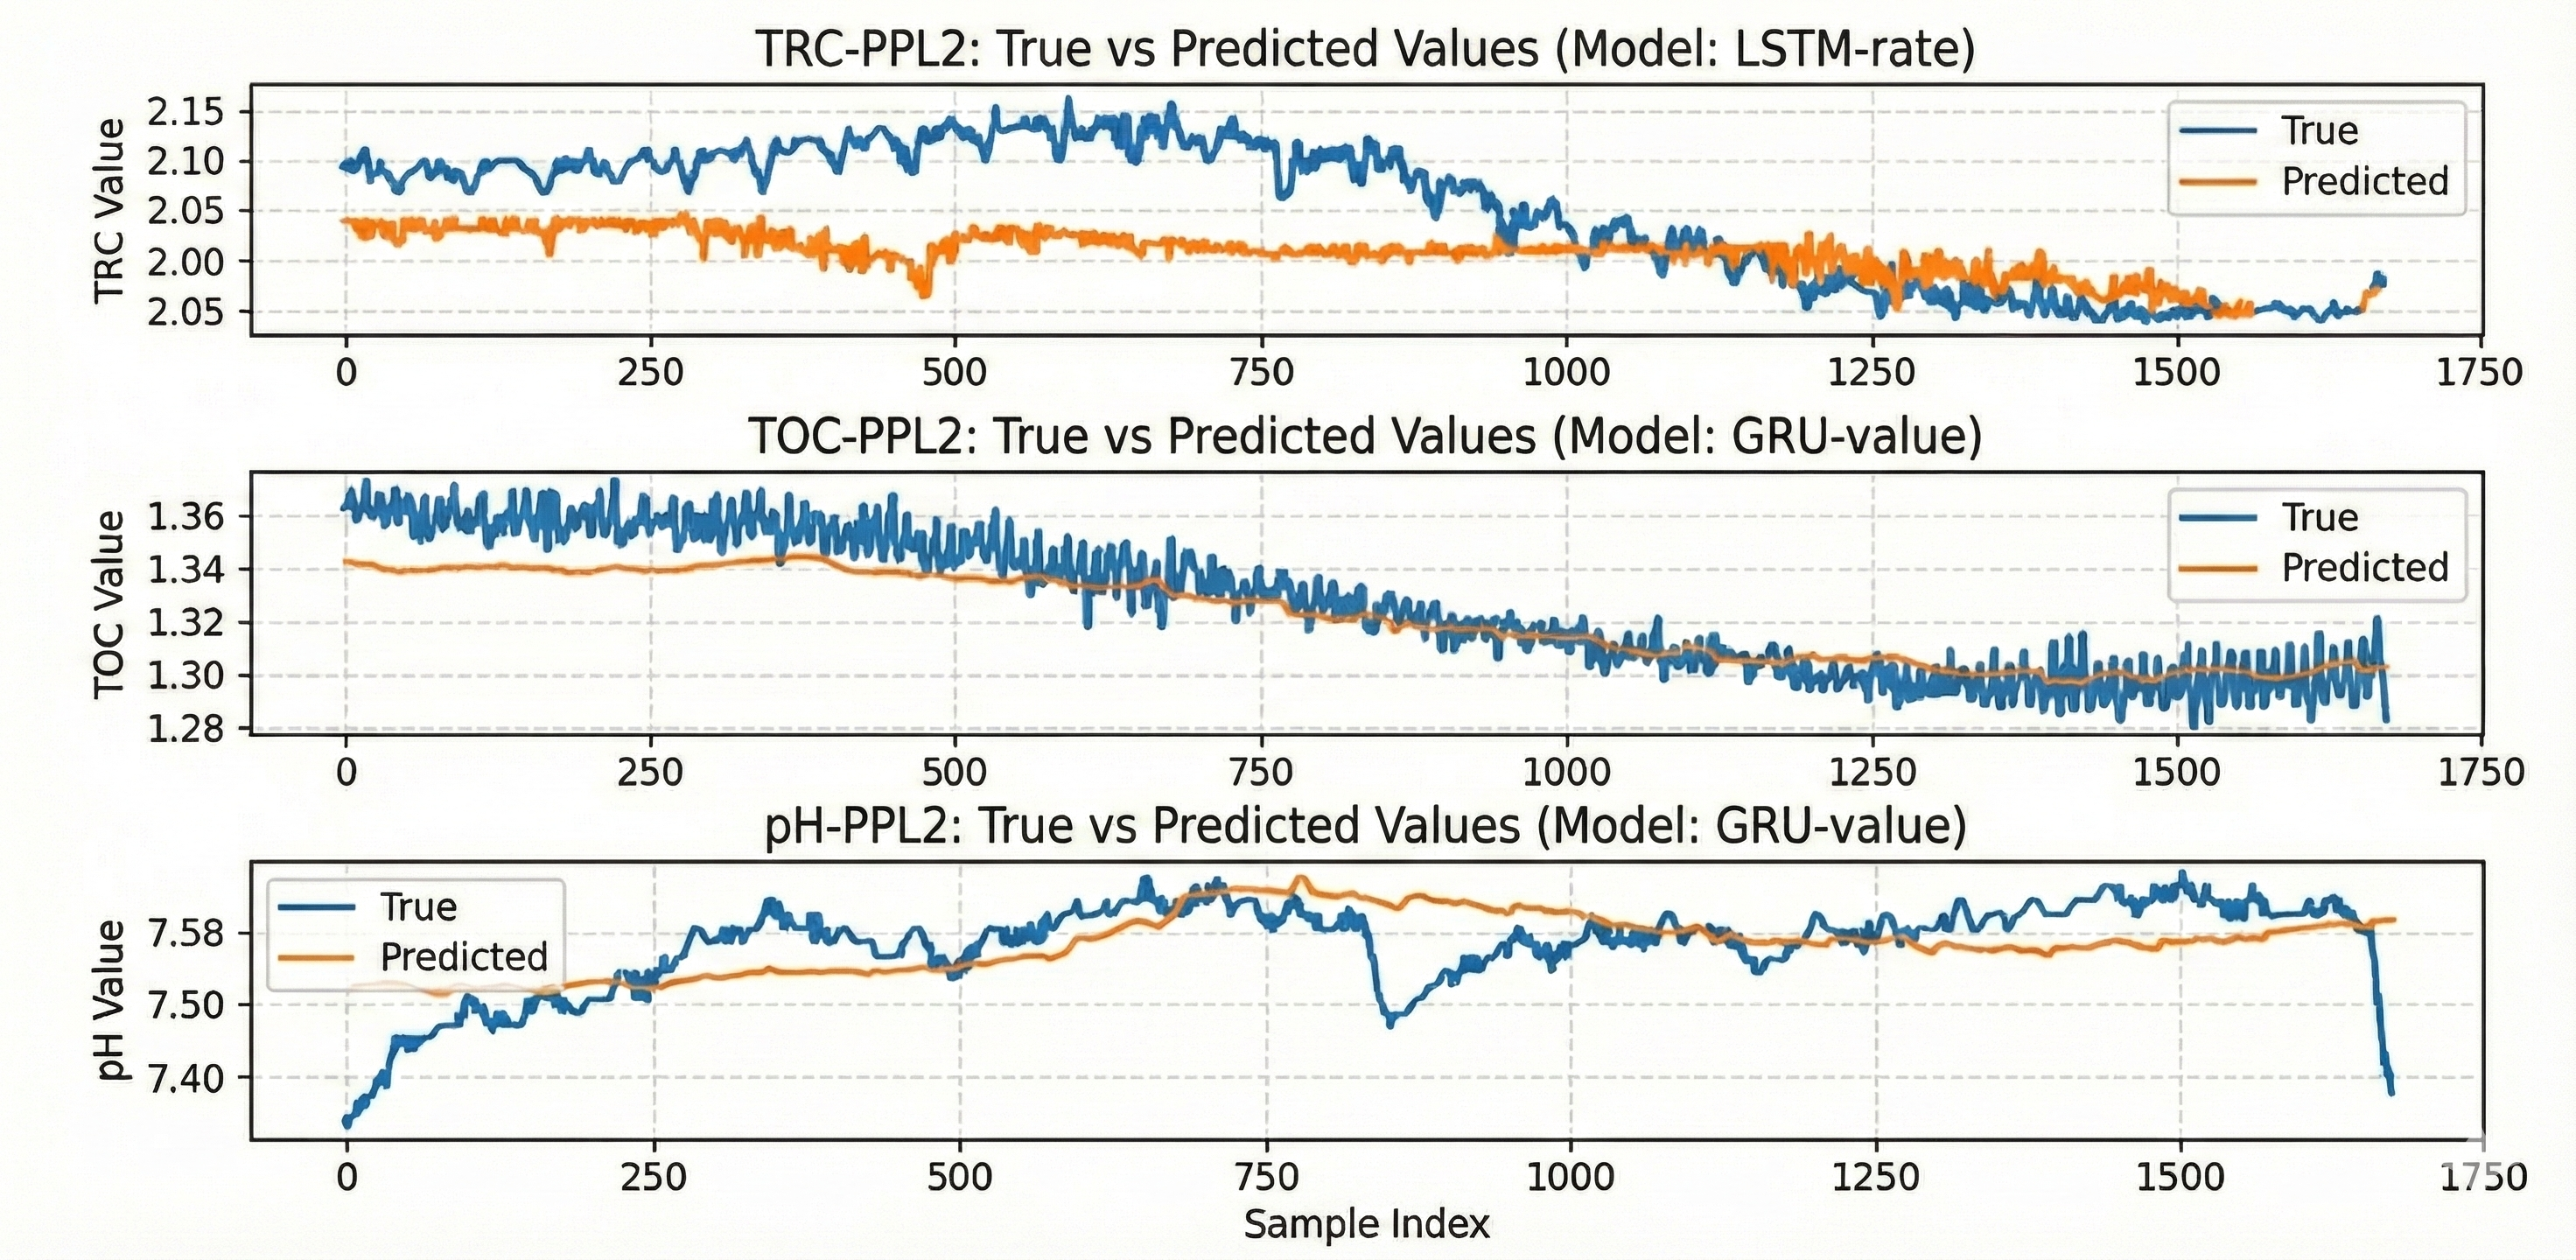
\includegraphics[width=\textwidth]{../attachment/midterm result plots.png}
    \caption{Comparison of predicted vs. actual values for the best-performing models (TRC, pH, and TOC) over a representative time segment.}
    \label{fig:results_plots}
\end{figure}

The results indicate that the choice of regression target—either the absolute value or the normalized rate of change—is critical and parameter-dependent. For Total Residual Chlorine (TRC), models trained on the normalized rate of change (e.g., LSTM-Rate) consistently outperformed those trained on absolute values, suggesting that focusing on the subtle dynamics of chlorine decay is a more effective strategy. Conversely, for pH and Total Organic Carbon (TOC), direct regression on the measured values yielded significantly better results. This implies that for these parameters, the absolute concentration is more directly predictable from the input features.

Among the different architectures, recurrent models, particularly LSTM and GRU, demonstrated strong performance across the board. The GRU-Value model emerged as the top performer for both pH and TOC, while the LSTM-Rate model was the best for TRC prediction in terms of Mean Squared Error. This highlights the suitability of these memory-based architectures for capturing the temporal dependencies inherent in water quality time-series data.

\section{Conclusion}
This study successfully demonstrated the potential of deep learning models for predicting water quality parameters in a distribution system. By leveraging high-frequency sensor data, we established that recurrent neural networks, especially GRU and LSTM, are highly effective in capturing the complex temporal dynamics of water quality changes. The introduction of "rate" regression proved beneficial for TRC prediction, while direct value prediction worked best for pH and TOC. These findings provide a solid foundation for developing real-time monitoring and control systems to minimize DBP formation.

\section{Future Work}
Based on the progress to date, several future directions have been identified, as outlined in the experimental framework shown in Figure \ref{fig:exp_framework}.
\begin{itemize}
    \item \textbf{Expand Dataset:} Incorporate new data as it becomes available to increase the size and diversity of the training set, which is crucial for model generalization.
    \item \textbf{Enhance Optimization:} Increase the number of trials in the Bayesian optimization runs to allow for a more thorough exploration of the hyperparameter space, potentially yielding more optimal models.
    \item \textbf{Explore Advanced Models:} Investigate state-of-the-art time series models, such as the Transformer~\cite{vaswani2017attention} and its recent variants (e.g., iTransformer, PatchTST), which have shown strong performance on long-sequence forecasting tasks.
    \item \textbf{Model Interpretability:} Employ interpretability techniques such as SHAP (SHapley Additive exPlanations), PDP (Partial Dependence Plots), and LIME (Local Interpretable Model-agnostic Explanations) to understand the model's decision-making process. This will help identify which sensor features have the most significant impact on DBP formation predictions, providing valuable insights for water quality management.
    \item \textbf{Develop a Second-Stage DBP Model:} Create a subsequent model to establish a mapping from the predicted water quality parameters (TRC, TOC, pH) to actual DBP concentrations measured by offline laboratory instruments. This would achieve the ultimate goal of predicting specific DBP levels from sensor data.
\end{itemize}

\begin{figure}[h!]
    \centering
    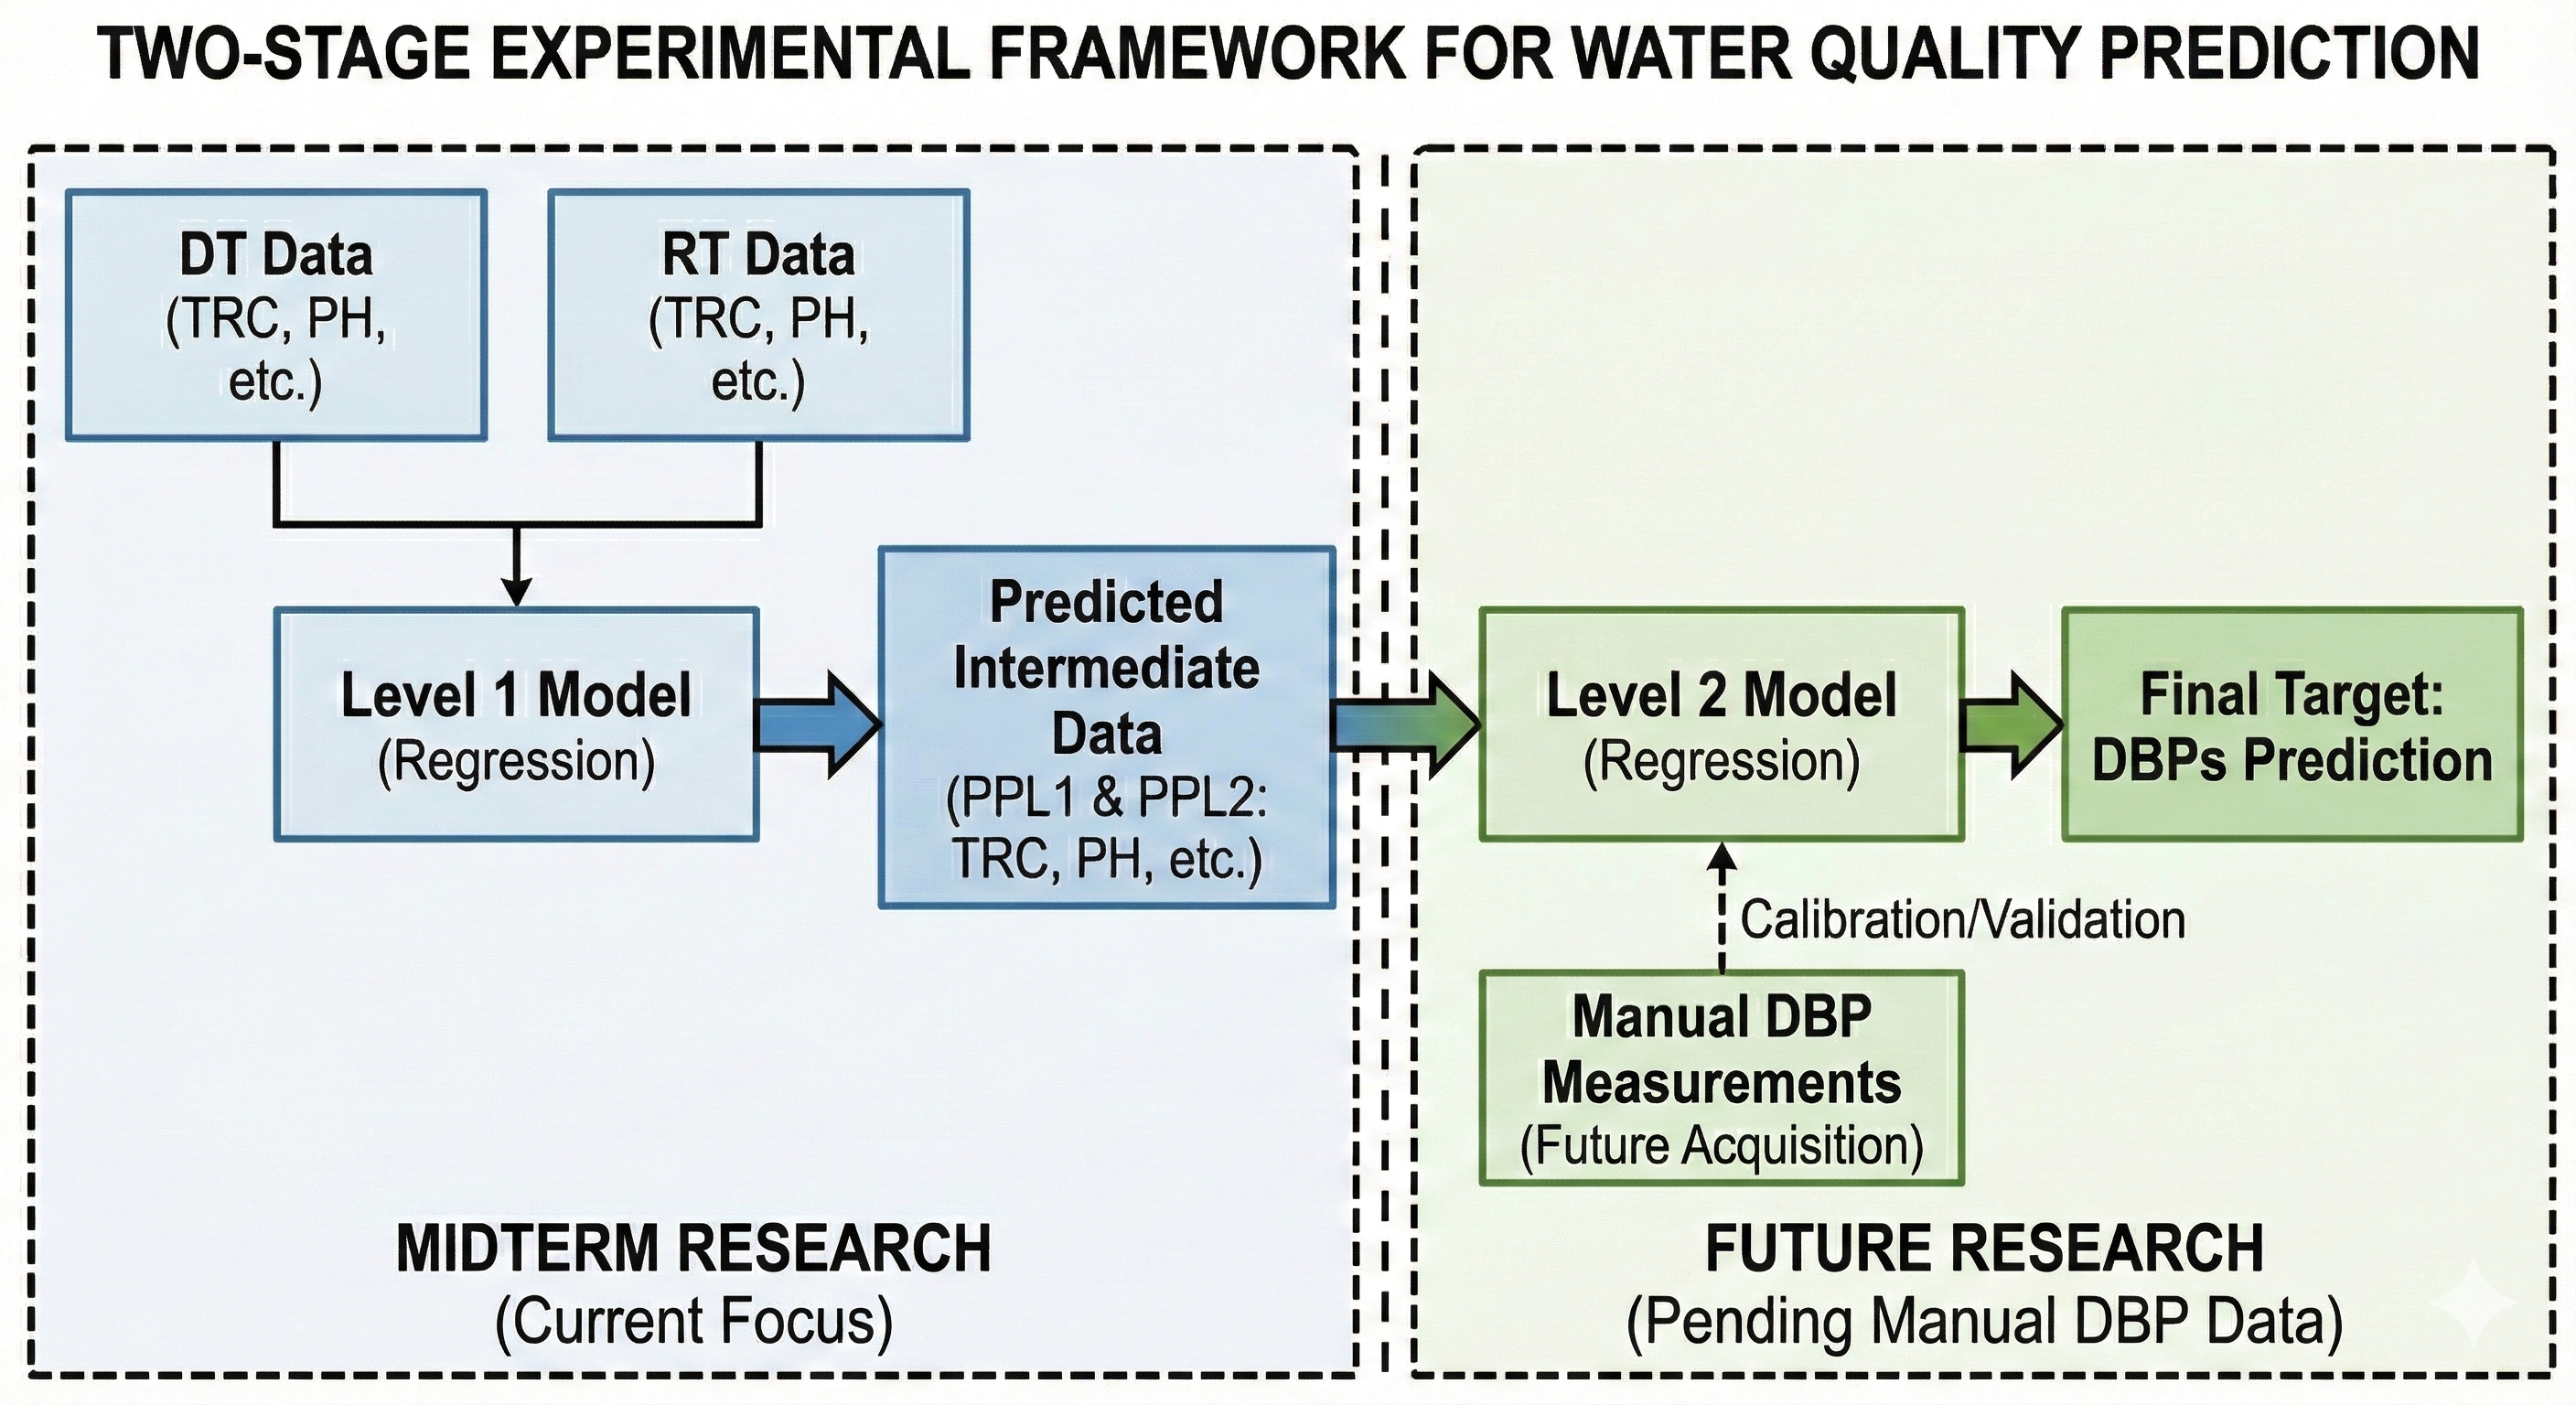
\includegraphics[width=\textwidth]{../attachment/experiment framework.png}
    \caption{The experimental framework guiding future work.}
    \label{fig:exp_framework}
\end{figure}

\bibliographystyle{unsrt}
\bibliography{references}

\end{document}